\documentclass[conference]{IEEEtran}
\usepackage[ruled,vlined]{algorithm2e}
\usepackage{amsmath}
\usepackage[english]{babel} %localisation
\usepackage{caption,subcaption} %supposedly incompatible with Springer and IOP, IEEETran and ACM SIG
\usepackage{cite} %nice citations, e.g. [1--5]
\usepackage{fixltx2e} %fix latex bugs
\usepackage{graphicx}
\PassOptionsToPackage{hyphens}{url}\usepackage{hyperref} %clickable URLS
\usepackage[htt]{hyphenat} %hyphenate \texttt
\usepackage{microtype} %makes text pretty; also condenses
\usepackage{multirow} %multiple rows in tables
\usepackage{siunitx,textcomp} %\SI{value}{unit}, \si{unit}; textcomp for microtype compatibility
%\usepackage [caption=false]{subfig} %if caption/subcaption not available
% \usepackage{tikz,pgfplots} %drawings and plots
\usepackage[siunitx]{circuitikz} %circuit figures
\usepackage[T1]{fontenc} %ensure proper hyphenation and treatment of math in sentences
\usepackage{booktabs}
\bibliographystyle{IEEEtran}

\usepackage{tikz}
\usepackage{verbatim}
\usepackage{listings}
\usepackage{pgfplots}
\begin{document}
\lstset{defaultdialect=[x86]{Assembler}}

% paper title
% can use linebreaks \\ within to get better formatting as desired
\title{Side Channel Analysis of an Embedded/Hardware Crypto Device}

% author names and affiliations
% use a multiple column layout for up to three different
% affiliations
\author{\IEEEauthorblockN{Sam Mitchell and Nathanael Weidler}
\IEEEauthorblockA{Deptartment of Electrical and Computer Engineering\\
Utah Stat University\\
Logan, Utah 84322\\
e-mail: samuel.alan.mitchell@gmail.com, NWeidler@gmail.com}
}

% make the title area
\maketitle


\begin{abstract}
%\boldmath
% Summarize project and results (executive summary).
%
This paper describes a side channel analysis attack on a microprocessor.  The microprocessor is running a Data Encryption Standard (DES) algorithm.  The goal of the attack is to recover the secret key from the device.  This is done by capturing the power usage of the device and using differential power analysis to analyze the data. 
 
\end{abstract}

\begin{IEEEkeywords}
Data Encryption Standard, Differential Power Analysis, Correlation Power Analysis, Security.
\end{IEEEkeywords}

\section{Introduction}
	Side channel analysis is one way to attack even the most computationally complex cryptographic devices.  Through side channel analysis, information (such as secret keys) can be obtained from devices without using more traditional or brute force attacks.  In order to carry out a side channel analysis attack, the attacker must have access to the device.  The attacker then obtains power information using an oscilloscope connected to a resistor put in series with the device's power input.

	In this paper a side channel analysis will be carried out on an Tiva-C  microprocessor to obtain the secret key from a Data Encryption Standard (DES) algorithm.  First, a typical DES implementation was written and loaded into the flash of the Tiva-C microprocessor.  Next, the side channel analysis was carried out.  After the power information, or traces, were obtained, a technique called differential power analysis (DPA) was used to analyze the data.  Another analysis using correlation power analysis was also carried out.  \cite{des} \cite{Messerges}


\subsection{Structure of paper}
	The organization is as follows: in Section \ref{sec::des_impl}, the development of the DES implementation is presented.  In Section \ref{sec::expr} the experimental test setup for the capturing of the traces is described. Section \ref{sec::analysis} contains the analysis of the data.  Conclusions are detailed in Section \ref{sec::conclusion}. 


\section{DES Implementation} \label{sec::des_impl}
	As a part of this work an implementation of DES was written for the Tiva-C microprocessor.  "The DES Algorith Illustrated" was a valuable resource during this process.  All of the explicit details of DES will be left to other work, however, a brief overview will be presented in order for the reader to grasp the complexity of the algorithm. \cite{des}

	DES is a 16 round encryption algorithm.  It works on 64-bit blocks of plaintext and outputs encrypted data of the same size.  The output of the algorithm is the cipher text.  The first step in DES is to divide the plaintext block in half, the left 32-bits and the right 32-bits.  The heart of DES is the 56-bit master key which is used to create 16 distinct 48-bit round keys, one for each round of the algorithm.  (The intent of this attack is to recover the key from the 16th round, from which all other keys can be easily obtained.)  To create each round key the 56-bit key is permuted and divided into two halves.  Then for each round each of those halves is shifted, recombined and permuted yielding the 48-bit round keys.

	One half of the plaintext (32-bits) is expanded and permuted to create a 48-bit word which is xored with the round key.  The result is divided into 8 6-bit parts which go through 8 distinct s-boxes.  An s-box is  method to substitute a 6-bit input with a 4-bit output.  These 4-bit outputs are put back together and permuted to create a 32-bit word which is xored with the other half of the plaintext.  This process is repeated 16 times until finally the two halves are put back together and permuted one last time to create the cipher text.  An illustration of one round is shown in figure \ref{fig:round}.

	\begin{figure}[h]
	\centering
	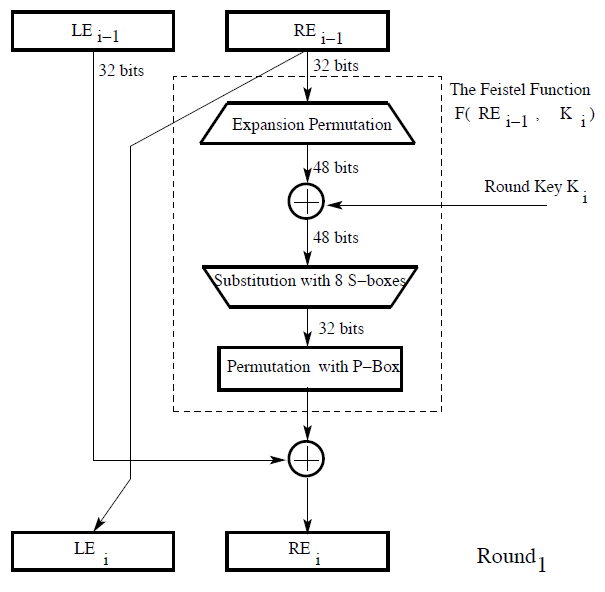
\includegraphics[width=0.7\linewidth]{./round}
	\caption{One round of DES.}
	\label{fig:round}
	\end{figure}

\subsection{DES Modifications}
	In order to facilitate the process by which traces are obtained, there was an addition to the traditional DES algorithm.  This slight modification in no way compromises the integrity of the algorithm or its outputs.  The change was to hold a general purpose input/output (GPIO) high during the algorithm except during a single instruction in which the output of the Feistel function is xored with the other half of the plaintext in round 16 and the result is written back to a register.  This allowed an oscilloscope to be triggered on the falling edge of the GPIO and frame this critical step which will be discussed later.  There were also two no-operations (nops) added before this register write and one after to allow the GPIO to settle and facilitate a cleaner capture.  The output of the assembly dump with comments added can be seen in figure \ref{fig:asm_snippet}.  Note that the register where the xor is written to (R0) is set to zero before the output of the xor is written there.
	
	\begin{figure}[h]
	\centering
	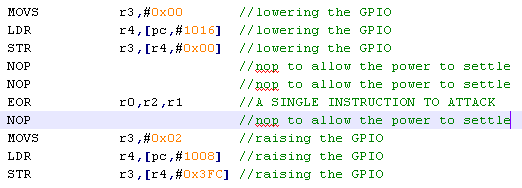
\includegraphics[width=0.7\linewidth]{./asm_snippet}
	\caption{The assembly showing the GPIO writes surrounding the xor and register write under attack.}
	\label{fig:asm_snippet}
	\end{figure}

	

\section{Experimental Setup} \label{sec::expr}
	This portion of the experiment was the most crucial to its success.  The goal is to obtain information about the power usage of the microprocessor during a critical step of the DES algorithm.  During a register write operation the power used will be different depending on the value of the word written.  It is believed that by analyzing this information, the secret key to the algorithm can be obtained.
	
	The oscilloscope used was a Techtronix DP0-2024 the sample rate was 1Gs per second and each trace contained about 270 samples.  The Tiva-C used a 17 MHz clock so there 38.5 samples per clock.
	
	The setup used involved the Tiva-C microprocessor powered by a bench top power supply through a breadboard.  The ground connection between the microprocessor and the power supply had a 1-$\Omega$ resistor added in series.  An Oscilloscope probe was placed on the resistor so that the voltage could be measured.  Then another oscilloscope probe was placed on the GPIO pin discussed in the previous section to act as the trigger.  The voltage data would be taken twenty times for each plain text value used in the DES algorithm and then averaged in an attempt to reduce noise.  91,840 captures with 4,592 unique plain text values would be obtained.  Each trace takes about two seconds to capture so the time to obtain all traces is 183,680 seconds or about 51 hours.  The voltage data acquired would be analyzed later to determine the secret key.  The test setup is illustrated in figure \ref{fig:bench}

	\begin{figure}[h]
	\centering
	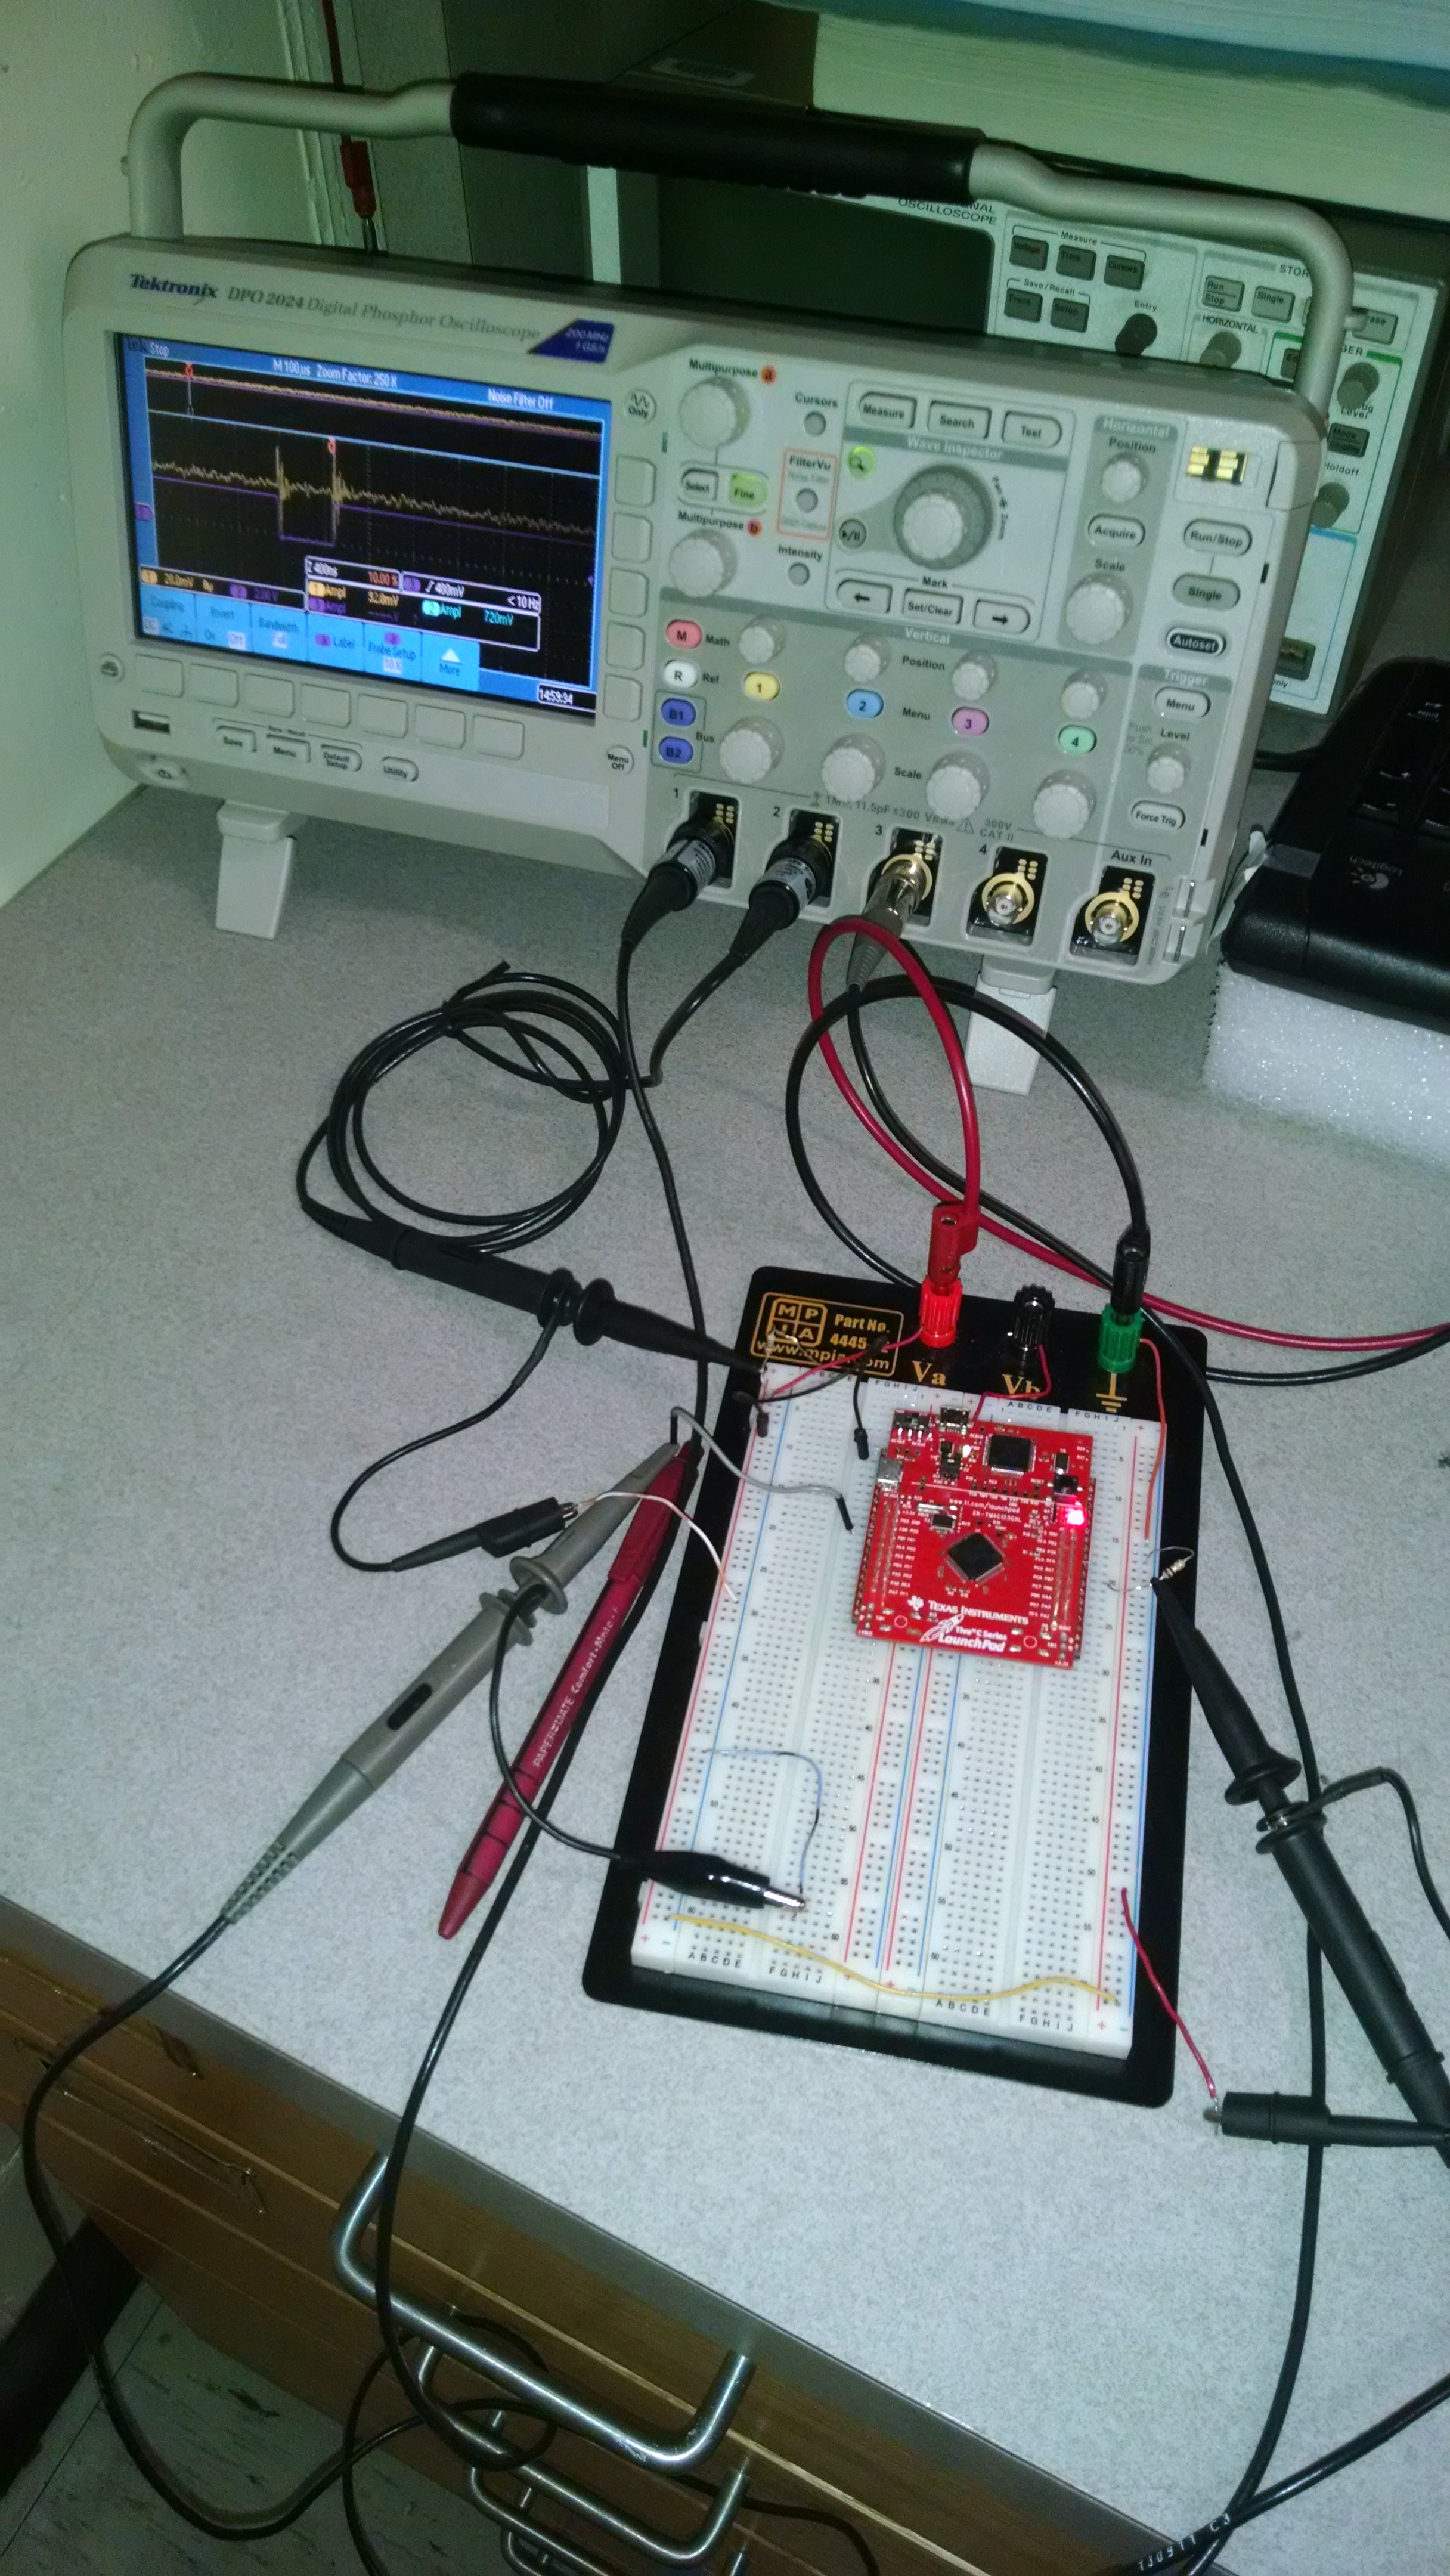
\includegraphics[width=0.7\linewidth]{./bench}
	\caption{Test setup showing the oscilloscope connected to the Tiva-C board.}
	\label{fig:bench}
	\end{figure}
	
	The test setup needed to be automated to facilitate the capturing of the traces.  In order for this to be done a matlab file was written to interface with the oscilloscope.  As trivial as this may sound it was not easy.  It took many hours of learning the oscilloscope and the commands to control it through matlab.  It also took time and patience to fine tune the DES implementation to create enough delay between each run of the algorithm to allow for the oscilloscope to transfer the data capture and re-arm itself.
	

\section{Analysis of the Data}\label{sec::analysis} 
\subsection{Differential Power Analysis}
	In order to analyze the data, differential power analysis (DPA) was employed.  Round 16 was chosen for this because given the cipher text, the input to the Feistel function and the output from the second xor (seen in the bottom right of figure \ref{fig:round}) can be determined.  Then the round key is guessed 6 bits at a time.  This greatly reduces the complexity of the key as there are only 64 possible combinations for a guess of 6 bits of the key.  Using knowledge of the Feistel function and the 6-bit key guess, the output of the Feistel function can be guessed at 4 bits at a time.  Remember, the s-boxes reduce the data from 48 bits to 32 bits.  This output is xored with the D value, and we already know the output of this xor.  So guessing one input and knowing the output determines the other input to the xor gate.  

	For each key guess 4-bits of the D word are deduced.  These 4-bit groups are divided into 3 sets where set 0 contains all guesses for which the four bits guessed are "0000," set 1 contains all guess where the 4 bits are "1111," and set 2 contains all other guessed values.  The average power for each sample point for sets 0 and 1 is calculated.  The two average powers are subtracted from each other.  The correct key guess will show large spikes where the calculation was actually made on the trace.  This is where the difference between the 2 sets of data is the greatest.  This process is repeated 8 times, once for each s-box until the correct key is determined.

 	 Figures \ref{fig:dpa1} through \ref{fig:dpa8} in Apendix A show the outputs of the DPA.  Unfortunately, none of the key values were able to be recovered based on DPA.  More discussion of this to follow.

\subsection{Correlation Power Analysis}
  Correlation Power Analysis (CPA) was also used on the data captured to see if more clear results could be obtained than what DPA provided.  In CPA the guessed at D word is sorted using the hamming distance of the change in the register value.  I our case the register was always set to 0 prior to the calculation, so in this case the Hamming distance is the same as the Hamming weight of the result.  Hamming weight is the number of 1s a data word contains.  The Hamming distance is the number bit changes from one word to the next so you count the number of 0s that changed to 1s and add that number to the number of 1s that changed to 0s.  The Hamming distance of anything from 0 is the Hamming weight of the data word.
  Each sample from every trace is entered into Pearson's sample correlation coefficient along with the Hamming weight of the guess.  The result should show a high correlation for the correct key guess.  The key guesses are the same 6-bit key guesses that were used in the DPA attack.
  The finest resolution the oscilloscope showed was 20$mV$/div. The bulk of the traces had nominal values of 4$mV$, with fluctuations of $\pm 5mV$. The oscilloscope has 8-bit resolution, which translates to a resolution of $0.1mV$. By using such low resolution, the representation of the significant portion of the signal (the xor operation) is reduced to 12 values or 4 bits. The error introduced by discretization could be one reason for inaccurate reading of the system. As an illustration of this, Figure \ref{fig:res} shows the measurement error between traces with matching plaintexts. 

	\begin{figure}[h]
	% This file was created by matlab2tikz.
% Minimal pgfplots version: 1.3
%
%The latest updates can be retrieved from
%  http://www.mathworks.com/matlabcentral/fileexchange/22022-matlab2tikz
%where you can also make suggestions and rate matlab2tikz.
%
\definecolor{mycolor1}{rgb}{0.00000,0.75000,0.75000}%
\definecolor{mycolor2}{rgb}{0.75000,0.00000,0.75000}%
\definecolor{mycolor3}{rgb}{0.75000,0.75000,0.00000}%
%
\begin{tikzpicture}

\begin{axis}[%
width=4.822222in,
height=3.631278in,
at={(0.808889in,0.490111in)},
scale only axis,
separate axis lines,
every outer x axis line/.append style={black},
every x tick label/.append style={font=\color{black}},
xmin=63.1353245317378,
xmax=85.1054402965661,
xlabel={Time (Samples)},
every outer y axis line/.append style={black},
every y tick label/.append style={font=\color{black}},
ymin=0.00331700379266751,
ymax=0.00478982300884956,
ylabel={Voltage (mV)},
title={Measurement resolution}
]
\addplot [color=blue,solid,forget plot]
  table[row sep=crcr]{%
50	0.00472\\
51	0.0048\\
52	0.00448\\
53	0.004\\
54	0.0036\\
55	0.00328\\
56	0.00312\\
57	0.00336\\
58	0.00376\\
59	0.004\\
60	0.00384\\
61	0.00368\\
62	0.00368\\
63	0.00384\\
64	0.004\\
65	0.0044\\
66	0.00456\\
67	0.00456\\
68	0.00456\\
69	0.00432\\
70	0.00408\\
71	0.00392\\
72	0.00384\\
73	0.00376\\
74	0.00368\\
75	0.00368\\
76	0.0036\\
77	0.00352\\
78	0.0036\\
79	0.00376\\
80	0.00392\\
81	0.00416\\
82	0.00432\\
83	0.00432\\
84	0.00432\\
85	0.00432\\
86	0.00416\\
87	0.00416\\
88	0.00408\\
89	0.004\\
90	0.004\\
91	0.00384\\
92	0.0036\\
93	0.00352\\
94	0.0036\\
95	0.00376\\
96	0.004\\
97	0.00416\\
98	0.00424\\
99	0.00432\\
100	0.00416\\
101	0.00408\\
102	0.00408\\
103	0.004\\
104	0.00392\\
105	0.00392\\
106	0.00376\\
107	0.00368\\
108	0.00352\\
109	0.00344\\
110	0.00352\\
111	0.00352\\
112	0.00352\\
113	0.00368\\
114	0.00376\\
115	0.00384\\
116	0.00392\\
117	0.00392\\
118	0.00392\\
119	0.00392\\
120	0.00392\\
121	0.004\\
122	0.004\\
123	0.004\\
124	0.004\\
125	0.004\\
126	0.00408\\
127	0.00416\\
128	0.00424\\
129	0.00432\\
130	0.0044\\
131	0.00448\\
132	0.0044\\
133	0.00432\\
134	0.00408\\
135	0.00408\\
136	0.004\\
137	0.004\\
138	0.004\\
139	0.00408\\
140	0.004\\
141	0.00408\\
142	0.00408\\
143	0.00416\\
144	0.00408\\
145	0.004\\
146	0.004\\
147	0.00408\\
148	0.00416\\
149	0.00424\\
150	0.00424\\
151	0.00424\\
152	0.00424\\
153	0.00416\\
154	0.00416\\
155	0.00416\\
156	0.00416\\
157	0.00408\\
158	0.004\\
159	0.004\\
160	0.004\\
161	0.004\\
162	0.004\\
163	0.00408\\
164	0.00416\\
165	0.00416\\
166	0.00416\\
167	0.00416\\
168	0.00416\\
169	0.00408\\
170	0.004\\
171	0.00392\\
172	0.00384\\
173	0.00384\\
174	0.00384\\
175	0.00392\\
176	0.00408\\
177	0.00408\\
178	0.004\\
179	0.004\\
180	0.00408\\
181	0.00416\\
182	0.00424\\
183	0.00416\\
184	0.00416\\
185	0.00416\\
186	0.00424\\
187	0.00432\\
188	0.00448\\
189	0.00448\\
190	0.00448\\
191	0.00448\\
192	0.00448\\
193	0.0044\\
194	0.00432\\
195	0.00424\\
196	0.00416\\
197	0.00392\\
198	0.00384\\
199	0.00384\\
200	0.00384\\
};
\addplot [color=black!50!green,solid,forget plot]
  table[row sep=crcr]{%
50	0.00432\\
51	0.00424\\
52	0.004\\
53	0.00368\\
54	0.00336\\
55	0.00312\\
56	0.00312\\
57	0.00328\\
58	0.0036\\
59	0.00376\\
60	0.00376\\
61	0.00368\\
62	0.00352\\
63	0.0036\\
64	0.00368\\
65	0.00384\\
66	0.00392\\
67	0.00392\\
68	0.00384\\
69	0.00368\\
70	0.00352\\
71	0.00336\\
72	0.00344\\
73	0.0036\\
74	0.00376\\
75	0.00376\\
76	0.00368\\
77	0.00368\\
78	0.00368\\
79	0.00384\\
80	0.004\\
81	0.00408\\
82	0.00416\\
83	0.00424\\
84	0.00408\\
85	0.004\\
86	0.004\\
87	0.00392\\
88	0.00392\\
89	0.00384\\
90	0.00384\\
91	0.00376\\
92	0.00376\\
93	0.00368\\
94	0.00368\\
95	0.00376\\
96	0.00392\\
97	0.00408\\
98	0.00408\\
99	0.00416\\
100	0.00416\\
101	0.00416\\
102	0.00416\\
103	0.00416\\
104	0.004\\
105	0.00392\\
106	0.00392\\
107	0.00384\\
108	0.00376\\
109	0.00376\\
110	0.00376\\
111	0.00384\\
112	0.00384\\
113	0.00384\\
114	0.00392\\
115	0.00392\\
116	0.00384\\
117	0.00384\\
118	0.00368\\
119	0.0036\\
120	0.00352\\
121	0.00352\\
122	0.0036\\
123	0.00352\\
124	0.00344\\
125	0.00344\\
126	0.00344\\
127	0.00344\\
128	0.00344\\
129	0.00352\\
130	0.0036\\
131	0.00368\\
132	0.00376\\
133	0.00376\\
134	0.00376\\
135	0.00376\\
136	0.00376\\
137	0.00368\\
138	0.0036\\
139	0.00352\\
140	0.00344\\
141	0.00344\\
142	0.00352\\
143	0.00352\\
144	0.0036\\
145	0.00376\\
146	0.00376\\
147	0.00384\\
148	0.00384\\
149	0.00392\\
150	0.00392\\
151	0.00376\\
152	0.00368\\
153	0.00368\\
154	0.00368\\
155	0.00368\\
156	0.00376\\
157	0.00384\\
158	0.00384\\
159	0.00384\\
160	0.00392\\
161	0.00392\\
162	0.00392\\
163	0.00384\\
164	0.00384\\
165	0.00384\\
166	0.00392\\
167	0.00376\\
168	0.00368\\
169	0.00368\\
170	0.00368\\
171	0.00376\\
172	0.00384\\
173	0.00392\\
174	0.00392\\
175	0.00392\\
176	0.00392\\
177	0.00392\\
178	0.00376\\
179	0.00384\\
180	0.00384\\
181	0.00392\\
182	0.004\\
183	0.00408\\
184	0.00408\\
185	0.00408\\
186	0.004\\
187	0.004\\
188	0.00392\\
189	0.00392\\
190	0.00384\\
191	0.00376\\
192	0.00368\\
193	0.0036\\
194	0.00352\\
195	0.00352\\
196	0.00352\\
197	0.00352\\
198	0.00344\\
199	0.00344\\
200	0.00352\\
};
\addplot [color=red,solid,forget plot]
  table[row sep=crcr]{%
50	0.00456\\
51	0.00456\\
52	0.00424\\
53	0.00384\\
54	0.00336\\
55	0.00304\\
56	0.00296\\
57	0.0032\\
58	0.0036\\
59	0.00384\\
60	0.00384\\
61	0.00384\\
62	0.00384\\
63	0.00376\\
64	0.00376\\
65	0.004\\
66	0.00416\\
67	0.00416\\
68	0.00408\\
69	0.00392\\
70	0.00376\\
71	0.00368\\
72	0.00376\\
73	0.00384\\
74	0.004\\
75	0.004\\
76	0.004\\
77	0.004\\
78	0.004\\
79	0.00408\\
80	0.00416\\
81	0.00424\\
82	0.00432\\
83	0.0044\\
84	0.0044\\
85	0.00432\\
86	0.00424\\
87	0.00424\\
88	0.00416\\
89	0.00408\\
90	0.004\\
91	0.00392\\
92	0.00392\\
93	0.00384\\
94	0.00376\\
95	0.00376\\
96	0.00376\\
97	0.00384\\
98	0.004\\
99	0.00408\\
100	0.00408\\
101	0.004\\
102	0.004\\
103	0.004\\
104	0.00392\\
105	0.00392\\
106	0.00384\\
107	0.00384\\
108	0.00376\\
109	0.00368\\
110	0.00368\\
111	0.00376\\
112	0.00384\\
113	0.00392\\
114	0.00392\\
115	0.00408\\
116	0.00416\\
117	0.00408\\
118	0.00408\\
119	0.004\\
120	0.004\\
121	0.004\\
122	0.00392\\
123	0.00392\\
124	0.00392\\
125	0.00392\\
126	0.004\\
127	0.00408\\
128	0.00424\\
129	0.00432\\
130	0.0044\\
131	0.00424\\
132	0.00424\\
133	0.00432\\
134	0.00424\\
135	0.00416\\
136	0.00408\\
137	0.00408\\
138	0.00408\\
139	0.00408\\
140	0.00408\\
141	0.004\\
142	0.00392\\
143	0.00392\\
144	0.00392\\
145	0.00392\\
146	0.00408\\
147	0.00416\\
148	0.00424\\
149	0.00432\\
150	0.00432\\
151	0.00432\\
152	0.00432\\
153	0.00424\\
154	0.00416\\
155	0.004\\
156	0.00384\\
157	0.00384\\
158	0.00392\\
159	0.00408\\
160	0.00416\\
161	0.00424\\
162	0.00424\\
163	0.00432\\
164	0.0044\\
165	0.0044\\
166	0.0044\\
167	0.0044\\
168	0.00432\\
169	0.00424\\
170	0.00416\\
171	0.00408\\
172	0.00408\\
173	0.00408\\
174	0.004\\
175	0.004\\
176	0.00392\\
177	0.004\\
178	0.004\\
179	0.004\\
180	0.00392\\
181	0.00392\\
182	0.00408\\
183	0.00416\\
184	0.00424\\
185	0.0044\\
186	0.0044\\
187	0.0044\\
188	0.00432\\
189	0.00416\\
190	0.00408\\
191	0.00408\\
192	0.00408\\
193	0.004\\
194	0.004\\
195	0.004\\
196	0.004\\
197	0.00408\\
198	0.00416\\
199	0.00408\\
200	0.00408\\
};
\addplot [color=mycolor1,solid,forget plot]
  table[row sep=crcr]{%
50	0.004\\
51	0.00424\\
52	0.00432\\
53	0.00416\\
54	0.00384\\
55	0.00344\\
56	0.00312\\
57	0.00296\\
58	0.00304\\
59	0.00328\\
60	0.00336\\
61	0.00344\\
62	0.00344\\
63	0.00344\\
64	0.00352\\
65	0.00376\\
66	0.004\\
67	0.00424\\
68	0.00432\\
69	0.00416\\
70	0.00384\\
71	0.0036\\
72	0.00352\\
73	0.00344\\
74	0.00344\\
75	0.00352\\
76	0.00352\\
77	0.00344\\
78	0.00344\\
79	0.00336\\
80	0.00336\\
81	0.00336\\
82	0.00352\\
83	0.00368\\
84	0.00376\\
85	0.00376\\
86	0.00368\\
87	0.00368\\
88	0.00352\\
89	0.00352\\
90	0.00352\\
91	0.00352\\
92	0.00352\\
93	0.00344\\
94	0.00352\\
95	0.0036\\
96	0.00368\\
97	0.00368\\
98	0.00376\\
99	0.00384\\
100	0.00384\\
101	0.00376\\
102	0.00376\\
103	0.00384\\
104	0.00384\\
105	0.00392\\
106	0.00392\\
107	0.00392\\
108	0.00392\\
109	0.00392\\
110	0.00392\\
111	0.00392\\
112	0.00392\\
113	0.00392\\
114	0.00392\\
115	0.00384\\
116	0.00376\\
117	0.00376\\
118	0.00368\\
119	0.00368\\
120	0.00368\\
121	0.0036\\
122	0.00352\\
123	0.0036\\
124	0.00368\\
125	0.00376\\
126	0.0036\\
127	0.00352\\
128	0.00352\\
129	0.00352\\
130	0.00352\\
131	0.00344\\
132	0.00344\\
133	0.00352\\
134	0.0036\\
135	0.00368\\
136	0.00368\\
137	0.00384\\
138	0.00384\\
139	0.00384\\
140	0.00376\\
141	0.0036\\
142	0.00352\\
143	0.00344\\
144	0.00336\\
145	0.00336\\
146	0.00336\\
147	0.00344\\
148	0.0036\\
149	0.00368\\
150	0.00384\\
151	0.00392\\
152	0.00384\\
153	0.00384\\
154	0.00384\\
155	0.00376\\
156	0.00368\\
157	0.00368\\
158	0.00368\\
159	0.00368\\
160	0.00368\\
161	0.00376\\
162	0.00376\\
163	0.00376\\
164	0.00376\\
165	0.00384\\
166	0.00384\\
167	0.00376\\
168	0.00368\\
169	0.00368\\
170	0.00368\\
171	0.00376\\
172	0.00376\\
173	0.00376\\
174	0.00376\\
175	0.00376\\
176	0.00376\\
177	0.00376\\
178	0.00376\\
179	0.00368\\
180	0.00368\\
181	0.00368\\
182	0.00376\\
183	0.00376\\
184	0.00376\\
185	0.00384\\
186	0.00384\\
187	0.00392\\
188	0.004\\
189	0.004\\
190	0.004\\
191	0.00392\\
192	0.00384\\
193	0.00384\\
194	0.00384\\
195	0.00376\\
196	0.00384\\
197	0.00376\\
198	0.00384\\
199	0.00392\\
200	0.00392\\
};
\addplot [color=mycolor2,solid,forget plot]
  table[row sep=crcr]{%
50	0.00432\\
51	0.00448\\
52	0.00456\\
53	0.0044\\
54	0.00416\\
55	0.00384\\
56	0.00368\\
57	0.00368\\
58	0.00384\\
59	0.004\\
60	0.00408\\
61	0.00408\\
62	0.004\\
63	0.00392\\
64	0.00392\\
65	0.004\\
66	0.00416\\
67	0.0044\\
68	0.00448\\
69	0.00432\\
70	0.00416\\
71	0.00392\\
72	0.00384\\
73	0.00384\\
74	0.004\\
75	0.00408\\
76	0.00408\\
77	0.00392\\
78	0.00384\\
79	0.00384\\
80	0.00384\\
81	0.004\\
82	0.00416\\
83	0.00424\\
84	0.00432\\
85	0.00424\\
86	0.00416\\
87	0.00408\\
88	0.004\\
89	0.004\\
90	0.004\\
91	0.00392\\
92	0.00392\\
93	0.00392\\
94	0.00384\\
95	0.00384\\
96	0.00392\\
97	0.00408\\
98	0.00424\\
99	0.00448\\
100	0.00448\\
101	0.0044\\
102	0.0044\\
103	0.0044\\
104	0.00432\\
105	0.00432\\
106	0.00424\\
107	0.00416\\
108	0.00408\\
109	0.00384\\
110	0.00384\\
111	0.00376\\
112	0.00376\\
113	0.00392\\
114	0.00416\\
115	0.00424\\
116	0.00432\\
117	0.00424\\
118	0.00424\\
119	0.00424\\
120	0.00424\\
121	0.00416\\
122	0.00408\\
123	0.00416\\
124	0.00424\\
125	0.00424\\
126	0.00416\\
127	0.00408\\
128	0.00408\\
129	0.00416\\
130	0.00424\\
131	0.00432\\
132	0.00432\\
133	0.00432\\
134	0.00432\\
135	0.00432\\
136	0.00424\\
137	0.00416\\
138	0.004\\
139	0.00392\\
140	0.00392\\
141	0.00392\\
142	0.00392\\
143	0.004\\
144	0.004\\
145	0.00408\\
146	0.00416\\
147	0.00416\\
148	0.00416\\
149	0.00432\\
150	0.0044\\
151	0.0044\\
152	0.0044\\
153	0.0044\\
154	0.00432\\
155	0.00408\\
156	0.00384\\
157	0.00376\\
158	0.00376\\
159	0.00376\\
160	0.00384\\
161	0.00392\\
162	0.00392\\
163	0.004\\
164	0.004\\
165	0.00392\\
166	0.00384\\
167	0.00384\\
168	0.00392\\
169	0.00392\\
170	0.004\\
171	0.00408\\
172	0.00408\\
173	0.00416\\
174	0.00416\\
175	0.00416\\
176	0.00408\\
177	0.00384\\
178	0.00384\\
179	0.00376\\
180	0.00376\\
181	0.00368\\
182	0.00376\\
183	0.00376\\
184	0.00392\\
185	0.00392\\
186	0.00392\\
187	0.00392\\
188	0.004\\
189	0.004\\
190	0.00408\\
191	0.00424\\
192	0.00432\\
193	0.0044\\
194	0.0044\\
195	0.0044\\
196	0.0044\\
197	0.0044\\
198	0.00432\\
199	0.00424\\
200	0.00424\\
};
\addplot [color=mycolor3,solid,forget plot]
  table[row sep=crcr]{%
50	0.004\\
51	0.00408\\
52	0.00392\\
53	0.00368\\
54	0.00336\\
55	0.00312\\
56	0.00304\\
57	0.00304\\
58	0.00328\\
59	0.00352\\
60	0.00368\\
61	0.00368\\
62	0.0036\\
63	0.0036\\
64	0.00376\\
65	0.00392\\
66	0.00416\\
67	0.00416\\
68	0.00416\\
69	0.00408\\
70	0.00392\\
71	0.00376\\
72	0.00376\\
73	0.00376\\
74	0.00392\\
75	0.00392\\
76	0.00392\\
77	0.00392\\
78	0.00384\\
79	0.00384\\
80	0.00384\\
81	0.00384\\
82	0.004\\
83	0.00408\\
84	0.00408\\
85	0.004\\
86	0.004\\
87	0.00392\\
88	0.00392\\
89	0.00384\\
90	0.00376\\
91	0.0036\\
92	0.00344\\
93	0.00344\\
94	0.00344\\
95	0.00336\\
96	0.00344\\
97	0.00352\\
98	0.0036\\
99	0.0036\\
100	0.00376\\
101	0.00368\\
102	0.00368\\
103	0.00368\\
104	0.00376\\
105	0.00368\\
106	0.0036\\
107	0.00352\\
108	0.00344\\
109	0.00344\\
110	0.00344\\
111	0.00352\\
112	0.0036\\
113	0.00368\\
114	0.00368\\
115	0.00376\\
116	0.00376\\
117	0.00376\\
118	0.00384\\
119	0.00392\\
120	0.00392\\
121	0.00384\\
122	0.00384\\
123	0.00376\\
124	0.00376\\
125	0.00376\\
126	0.0036\\
127	0.00352\\
128	0.00352\\
129	0.00368\\
130	0.00368\\
131	0.00384\\
132	0.00392\\
133	0.004\\
134	0.00408\\
135	0.00416\\
136	0.00424\\
137	0.00424\\
138	0.00424\\
139	0.00408\\
140	0.004\\
141	0.00392\\
142	0.00392\\
143	0.00384\\
144	0.00376\\
145	0.00376\\
146	0.00376\\
147	0.00384\\
148	0.00392\\
149	0.00392\\
150	0.00392\\
151	0.004\\
152	0.00392\\
153	0.00384\\
154	0.00384\\
155	0.00376\\
156	0.00368\\
157	0.00368\\
158	0.00368\\
159	0.00376\\
160	0.00376\\
161	0.00376\\
162	0.00376\\
163	0.00384\\
164	0.004\\
165	0.00408\\
166	0.00416\\
167	0.00408\\
168	0.00408\\
169	0.00408\\
170	0.00408\\
171	0.00408\\
172	0.00408\\
173	0.004\\
174	0.004\\
175	0.00392\\
176	0.00392\\
177	0.00392\\
178	0.00392\\
179	0.00392\\
180	0.00384\\
181	0.00384\\
182	0.00376\\
183	0.00376\\
184	0.00376\\
185	0.00376\\
186	0.00384\\
187	0.00384\\
188	0.00376\\
189	0.00368\\
190	0.0036\\
191	0.00368\\
192	0.0036\\
193	0.00344\\
194	0.00344\\
195	0.00352\\
196	0.0036\\
197	0.00368\\
198	0.00368\\
199	0.00376\\
200	0.00376\\
};
\addplot [color=darkgray,solid,forget plot]
  table[row sep=crcr]{%
50	0.00408\\
51	0.00416\\
52	0.004\\
53	0.0036\\
54	0.00328\\
55	0.00304\\
56	0.00312\\
57	0.0032\\
58	0.00344\\
59	0.00376\\
60	0.00392\\
61	0.00384\\
62	0.00368\\
63	0.00368\\
64	0.00368\\
65	0.00384\\
66	0.00392\\
67	0.00408\\
68	0.00408\\
69	0.004\\
70	0.00376\\
71	0.00352\\
72	0.00352\\
73	0.0036\\
74	0.00384\\
75	0.00392\\
76	0.004\\
77	0.00392\\
78	0.00368\\
79	0.0036\\
80	0.00368\\
81	0.00376\\
82	0.00384\\
83	0.00384\\
84	0.00384\\
85	0.00384\\
86	0.00376\\
87	0.00368\\
88	0.00368\\
89	0.00368\\
90	0.00368\\
91	0.0036\\
92	0.00352\\
93	0.00352\\
94	0.0036\\
95	0.00376\\
96	0.00392\\
97	0.004\\
98	0.00408\\
99	0.00416\\
100	0.00416\\
101	0.00416\\
102	0.00408\\
103	0.004\\
104	0.00376\\
105	0.00368\\
106	0.0036\\
107	0.0036\\
108	0.0036\\
109	0.0036\\
110	0.00368\\
111	0.00376\\
112	0.00392\\
113	0.004\\
114	0.00408\\
115	0.00408\\
116	0.00392\\
117	0.00384\\
118	0.00384\\
119	0.00384\\
120	0.00384\\
121	0.00384\\
122	0.004\\
123	0.00416\\
124	0.00416\\
125	0.004\\
126	0.00392\\
127	0.00384\\
128	0.00376\\
129	0.00384\\
130	0.00392\\
131	0.00408\\
132	0.00408\\
133	0.00408\\
134	0.00408\\
135	0.00416\\
136	0.00416\\
137	0.00416\\
138	0.00416\\
139	0.00416\\
140	0.00408\\
141	0.004\\
142	0.004\\
143	0.004\\
144	0.00408\\
145	0.00416\\
146	0.00424\\
147	0.00424\\
148	0.00424\\
149	0.00416\\
150	0.00416\\
151	0.00416\\
152	0.00408\\
153	0.004\\
154	0.004\\
155	0.00392\\
156	0.00384\\
157	0.00392\\
158	0.00384\\
159	0.00384\\
160	0.00392\\
161	0.00392\\
162	0.00392\\
163	0.00392\\
164	0.00392\\
165	0.004\\
166	0.00408\\
167	0.00408\\
168	0.00416\\
169	0.00408\\
170	0.00408\\
171	0.00408\\
172	0.004\\
173	0.00392\\
174	0.00392\\
175	0.00392\\
176	0.00392\\
177	0.00392\\
178	0.00392\\
179	0.00392\\
180	0.00392\\
181	0.00392\\
182	0.00384\\
183	0.00376\\
184	0.00384\\
185	0.00392\\
186	0.00392\\
187	0.00392\\
188	0.00384\\
189	0.00376\\
190	0.00376\\
191	0.00376\\
192	0.00376\\
193	0.00384\\
194	0.00384\\
195	0.00376\\
196	0.00384\\
197	0.00392\\
198	0.00408\\
199	0.00424\\
200	0.00432\\
};
\addplot [color=blue,solid,forget plot]
  table[row sep=crcr]{%
50	0.00448\\
51	0.00456\\
52	0.00432\\
53	0.00392\\
54	0.00352\\
55	0.00328\\
56	0.00328\\
57	0.00336\\
58	0.0036\\
59	0.00384\\
60	0.00392\\
61	0.004\\
62	0.004\\
63	0.00384\\
64	0.00392\\
65	0.00416\\
66	0.00424\\
67	0.00432\\
68	0.00432\\
69	0.00416\\
70	0.00392\\
71	0.00376\\
72	0.00368\\
73	0.00376\\
74	0.00392\\
75	0.004\\
76	0.00392\\
77	0.00384\\
78	0.00392\\
79	0.00392\\
80	0.004\\
81	0.004\\
82	0.00408\\
83	0.00416\\
84	0.00408\\
85	0.00384\\
86	0.00368\\
87	0.00368\\
88	0.0036\\
89	0.00352\\
90	0.00352\\
91	0.0036\\
92	0.0036\\
93	0.00368\\
94	0.00376\\
95	0.00384\\
96	0.004\\
97	0.004\\
98	0.00408\\
99	0.00408\\
100	0.00408\\
101	0.00408\\
102	0.00408\\
103	0.00408\\
104	0.004\\
105	0.00384\\
106	0.00376\\
107	0.0036\\
108	0.00352\\
109	0.00344\\
110	0.00344\\
111	0.00344\\
112	0.00352\\
113	0.0036\\
114	0.0036\\
115	0.0036\\
116	0.0036\\
117	0.0036\\
118	0.00368\\
119	0.00368\\
120	0.00368\\
121	0.0036\\
122	0.0036\\
123	0.0036\\
124	0.00368\\
125	0.00368\\
126	0.00368\\
127	0.00376\\
128	0.00384\\
129	0.00392\\
130	0.00392\\
131	0.00392\\
132	0.00384\\
133	0.00384\\
134	0.00384\\
135	0.00376\\
136	0.00376\\
137	0.00368\\
138	0.0036\\
139	0.00368\\
140	0.00376\\
141	0.00392\\
142	0.00392\\
143	0.00384\\
144	0.00384\\
145	0.00376\\
146	0.00376\\
147	0.00376\\
148	0.00376\\
149	0.00376\\
150	0.00384\\
151	0.00392\\
152	0.00408\\
153	0.00416\\
154	0.00432\\
155	0.00432\\
156	0.00432\\
157	0.0044\\
158	0.00432\\
159	0.00432\\
160	0.00432\\
161	0.00424\\
162	0.00424\\
163	0.00416\\
164	0.00408\\
165	0.00408\\
166	0.004\\
167	0.004\\
168	0.00408\\
169	0.00408\\
170	0.00408\\
171	0.00408\\
172	0.004\\
173	0.004\\
174	0.00392\\
175	0.00384\\
176	0.00392\\
177	0.00392\\
178	0.00408\\
179	0.00416\\
180	0.00416\\
181	0.00416\\
182	0.00424\\
183	0.00408\\
184	0.00392\\
185	0.00368\\
186	0.00376\\
187	0.00392\\
188	0.00392\\
189	0.00392\\
190	0.00392\\
191	0.004\\
192	0.00408\\
193	0.00408\\
194	0.00408\\
195	0.00392\\
196	0.00384\\
197	0.00368\\
198	0.00376\\
199	0.00376\\
200	0.00376\\
};
\addplot [color=black!50!green,solid,forget plot]
  table[row sep=crcr]{%
50	0.00376\\
51	0.00384\\
52	0.00384\\
53	0.0036\\
54	0.00328\\
55	0.00296\\
56	0.00288\\
57	0.00304\\
58	0.00336\\
59	0.00376\\
60	0.00392\\
61	0.00392\\
62	0.00368\\
63	0.0036\\
64	0.00376\\
65	0.00408\\
66	0.00424\\
67	0.00432\\
68	0.00424\\
69	0.00408\\
70	0.00368\\
71	0.00344\\
72	0.00336\\
73	0.00344\\
74	0.0036\\
75	0.00376\\
76	0.00392\\
77	0.00392\\
78	0.00368\\
79	0.00368\\
80	0.00368\\
81	0.00368\\
82	0.0036\\
83	0.0036\\
84	0.00352\\
85	0.00336\\
86	0.0032\\
87	0.0032\\
88	0.00312\\
89	0.00304\\
90	0.00296\\
91	0.00296\\
92	0.00296\\
93	0.00296\\
94	0.00304\\
95	0.00312\\
96	0.00328\\
97	0.00336\\
98	0.00352\\
99	0.0036\\
100	0.00376\\
101	0.00376\\
102	0.00376\\
103	0.00376\\
104	0.00368\\
105	0.00352\\
106	0.00336\\
107	0.00336\\
108	0.00336\\
109	0.00344\\
110	0.00344\\
111	0.00352\\
112	0.0036\\
113	0.00376\\
114	0.00384\\
115	0.00384\\
116	0.00384\\
117	0.00368\\
118	0.00368\\
119	0.00368\\
120	0.00368\\
121	0.00368\\
122	0.00368\\
123	0.0036\\
124	0.00344\\
125	0.00336\\
126	0.00328\\
127	0.0032\\
128	0.00328\\
129	0.00336\\
130	0.00352\\
131	0.00368\\
132	0.00376\\
133	0.00392\\
134	0.00408\\
135	0.00408\\
136	0.00408\\
137	0.004\\
138	0.004\\
139	0.00384\\
140	0.00368\\
141	0.00352\\
142	0.00344\\
143	0.00344\\
144	0.00344\\
145	0.00352\\
146	0.00368\\
147	0.00368\\
148	0.00368\\
149	0.00368\\
150	0.0036\\
151	0.0036\\
152	0.0036\\
153	0.0036\\
154	0.0036\\
155	0.0036\\
156	0.00368\\
157	0.0036\\
158	0.00352\\
159	0.00352\\
160	0.00352\\
161	0.0036\\
162	0.0036\\
163	0.00368\\
164	0.00368\\
165	0.00368\\
166	0.00368\\
167	0.00368\\
168	0.00368\\
169	0.00368\\
170	0.00368\\
171	0.00376\\
172	0.00368\\
173	0.00368\\
174	0.0036\\
175	0.0036\\
176	0.00352\\
177	0.00352\\
178	0.00344\\
179	0.00336\\
180	0.00336\\
181	0.00344\\
182	0.00344\\
183	0.00344\\
184	0.00352\\
185	0.0036\\
186	0.0036\\
187	0.00352\\
188	0.00352\\
189	0.0036\\
190	0.0036\\
191	0.00368\\
192	0.00376\\
193	0.00384\\
194	0.00392\\
195	0.00392\\
196	0.00392\\
197	0.00384\\
198	0.00384\\
199	0.00384\\
200	0.00392\\
};
\addplot [color=red,solid,forget plot]
  table[row sep=crcr]{%
50	0.00424\\
51	0.00432\\
52	0.00424\\
53	0.004\\
54	0.0036\\
55	0.00328\\
56	0.00304\\
57	0.00312\\
58	0.0032\\
59	0.00352\\
60	0.00384\\
61	0.00392\\
62	0.00384\\
63	0.00368\\
64	0.00376\\
65	0.00392\\
66	0.00416\\
67	0.0044\\
68	0.00456\\
69	0.00448\\
70	0.0044\\
71	0.00416\\
72	0.004\\
73	0.004\\
74	0.00408\\
75	0.00408\\
76	0.00408\\
77	0.00408\\
78	0.004\\
79	0.00384\\
80	0.00368\\
81	0.00368\\
82	0.00368\\
83	0.00392\\
84	0.00392\\
85	0.00392\\
86	0.00384\\
87	0.00376\\
88	0.00376\\
89	0.00376\\
90	0.00376\\
91	0.00384\\
92	0.00384\\
93	0.00376\\
94	0.00368\\
95	0.00376\\
96	0.00392\\
97	0.00416\\
98	0.00432\\
99	0.0044\\
100	0.0044\\
101	0.0044\\
102	0.00424\\
103	0.00408\\
104	0.004\\
105	0.00392\\
106	0.00392\\
107	0.00392\\
108	0.00384\\
109	0.00384\\
110	0.00376\\
111	0.00376\\
112	0.00384\\
113	0.004\\
114	0.004\\
115	0.004\\
116	0.004\\
117	0.00392\\
118	0.00392\\
119	0.004\\
120	0.004\\
121	0.004\\
122	0.004\\
123	0.004\\
124	0.00384\\
125	0.00368\\
126	0.00352\\
127	0.00352\\
128	0.0036\\
129	0.00376\\
130	0.00392\\
131	0.004\\
132	0.00408\\
133	0.00408\\
134	0.00408\\
135	0.00408\\
136	0.00416\\
137	0.00432\\
138	0.00424\\
139	0.00424\\
140	0.00416\\
141	0.00408\\
142	0.00392\\
143	0.00392\\
144	0.00392\\
145	0.004\\
146	0.00416\\
147	0.00416\\
148	0.00416\\
149	0.00424\\
150	0.00432\\
151	0.0044\\
152	0.0044\\
153	0.0044\\
154	0.00424\\
155	0.00416\\
156	0.00408\\
157	0.004\\
158	0.00392\\
159	0.00384\\
160	0.00376\\
161	0.00368\\
162	0.0036\\
163	0.00368\\
164	0.00384\\
165	0.004\\
166	0.00408\\
167	0.00408\\
168	0.004\\
169	0.004\\
170	0.00392\\
171	0.00384\\
172	0.00392\\
173	0.00392\\
174	0.004\\
175	0.004\\
176	0.004\\
177	0.004\\
178	0.00408\\
179	0.004\\
180	0.004\\
181	0.00408\\
182	0.00408\\
183	0.004\\
184	0.00392\\
185	0.00392\\
186	0.00392\\
187	0.00384\\
188	0.00384\\
189	0.00376\\
190	0.00368\\
191	0.00368\\
192	0.00376\\
193	0.00384\\
194	0.004\\
195	0.00392\\
196	0.00392\\
197	0.004\\
198	0.00408\\
199	0.004\\
200	0.00408\\
};
\addplot [color=mycolor1,solid,forget plot]
  table[row sep=crcr]{%
50	0.00448\\
51	0.00456\\
52	0.00432\\
53	0.004\\
54	0.00368\\
55	0.00344\\
56	0.00328\\
57	0.00336\\
58	0.00368\\
59	0.00408\\
60	0.00432\\
61	0.00432\\
62	0.00424\\
63	0.00408\\
64	0.004\\
65	0.00408\\
66	0.00416\\
67	0.00424\\
68	0.00432\\
69	0.00408\\
70	0.00392\\
71	0.00376\\
72	0.00384\\
73	0.00384\\
74	0.004\\
75	0.00408\\
76	0.00408\\
77	0.00392\\
78	0.00368\\
79	0.00352\\
80	0.00368\\
81	0.00384\\
82	0.004\\
83	0.00424\\
84	0.00424\\
85	0.00424\\
86	0.00416\\
87	0.00408\\
88	0.00408\\
89	0.00416\\
90	0.00408\\
91	0.004\\
92	0.00392\\
93	0.00384\\
94	0.00384\\
95	0.00384\\
96	0.004\\
97	0.00408\\
98	0.00416\\
99	0.00416\\
100	0.00408\\
101	0.004\\
102	0.004\\
103	0.004\\
104	0.004\\
105	0.004\\
106	0.00392\\
107	0.00376\\
108	0.0036\\
109	0.00352\\
110	0.00336\\
111	0.00336\\
112	0.00336\\
113	0.00344\\
114	0.00352\\
115	0.0036\\
116	0.0036\\
117	0.00368\\
118	0.00368\\
119	0.00384\\
120	0.00384\\
121	0.00384\\
122	0.004\\
123	0.00408\\
124	0.00408\\
125	0.00408\\
126	0.00408\\
127	0.00416\\
128	0.00424\\
129	0.00416\\
130	0.00408\\
131	0.004\\
132	0.004\\
133	0.004\\
134	0.004\\
135	0.004\\
136	0.00384\\
137	0.00384\\
138	0.00376\\
139	0.00376\\
140	0.00376\\
141	0.00376\\
142	0.00368\\
143	0.00368\\
144	0.00368\\
145	0.00384\\
146	0.00384\\
147	0.00392\\
148	0.004\\
149	0.00392\\
150	0.00408\\
151	0.00408\\
152	0.00408\\
153	0.00408\\
154	0.004\\
155	0.004\\
156	0.004\\
157	0.004\\
158	0.00392\\
159	0.00384\\
160	0.00376\\
161	0.00376\\
162	0.00368\\
163	0.00368\\
164	0.00368\\
165	0.00368\\
166	0.00376\\
167	0.00384\\
168	0.00384\\
169	0.00392\\
170	0.00384\\
171	0.00384\\
172	0.00384\\
173	0.00384\\
174	0.00384\\
175	0.00392\\
176	0.004\\
177	0.00408\\
178	0.00408\\
179	0.00408\\
180	0.00416\\
181	0.00424\\
182	0.00416\\
183	0.00416\\
184	0.00416\\
185	0.00408\\
186	0.00408\\
187	0.00408\\
188	0.004\\
189	0.004\\
190	0.00392\\
191	0.00392\\
192	0.00384\\
193	0.00376\\
194	0.00368\\
195	0.00368\\
196	0.00368\\
197	0.00384\\
198	0.00384\\
199	0.00392\\
200	0.00384\\
};
\addplot [color=mycolor2,solid,forget plot]
  table[row sep=crcr]{%
50	0.00392\\
51	0.00416\\
52	0.00416\\
53	0.00384\\
54	0.00352\\
55	0.0032\\
56	0.00312\\
57	0.00312\\
58	0.00328\\
59	0.0036\\
60	0.00376\\
61	0.00384\\
62	0.00368\\
63	0.0036\\
64	0.0036\\
65	0.00384\\
66	0.00416\\
67	0.00432\\
68	0.00432\\
69	0.00432\\
70	0.00416\\
71	0.00408\\
72	0.00392\\
73	0.004\\
74	0.00416\\
75	0.00424\\
76	0.00424\\
77	0.00416\\
78	0.00408\\
79	0.00408\\
80	0.00416\\
81	0.00432\\
82	0.00456\\
83	0.00456\\
84	0.00464\\
85	0.00456\\
86	0.00448\\
87	0.00432\\
88	0.00416\\
89	0.00408\\
90	0.004\\
91	0.004\\
92	0.004\\
93	0.00392\\
94	0.00384\\
95	0.00392\\
96	0.004\\
97	0.00416\\
98	0.00416\\
99	0.00416\\
100	0.00416\\
101	0.00424\\
102	0.00424\\
103	0.00432\\
104	0.00424\\
105	0.00416\\
106	0.00416\\
107	0.00408\\
108	0.00392\\
109	0.00376\\
110	0.00368\\
111	0.0036\\
112	0.00368\\
113	0.00376\\
114	0.00392\\
115	0.00392\\
116	0.004\\
117	0.004\\
118	0.00392\\
119	0.00392\\
120	0.00392\\
121	0.00376\\
122	0.00376\\
123	0.00384\\
124	0.00384\\
125	0.00384\\
126	0.00384\\
127	0.00384\\
128	0.00384\\
129	0.00384\\
130	0.00376\\
131	0.00376\\
132	0.00392\\
133	0.00408\\
134	0.004\\
135	0.00392\\
136	0.00384\\
137	0.00368\\
138	0.00368\\
139	0.0036\\
140	0.00368\\
141	0.00368\\
142	0.00384\\
143	0.00384\\
144	0.00384\\
145	0.00376\\
146	0.00368\\
147	0.00368\\
148	0.0036\\
149	0.00368\\
150	0.00368\\
151	0.0036\\
152	0.0036\\
153	0.00368\\
154	0.00376\\
155	0.00384\\
156	0.00384\\
157	0.00384\\
158	0.00376\\
159	0.00376\\
160	0.00384\\
161	0.00384\\
162	0.00384\\
163	0.00384\\
164	0.00384\\
165	0.00384\\
166	0.00392\\
167	0.00392\\
168	0.00384\\
169	0.00384\\
170	0.00384\\
171	0.00384\\
172	0.00384\\
173	0.00384\\
174	0.00376\\
175	0.00376\\
176	0.00376\\
177	0.00376\\
178	0.00384\\
179	0.00376\\
180	0.00384\\
181	0.00384\\
182	0.00376\\
183	0.00376\\
184	0.00376\\
185	0.00376\\
186	0.00376\\
187	0.00376\\
188	0.00368\\
189	0.0036\\
190	0.00352\\
191	0.00352\\
192	0.00352\\
193	0.0036\\
194	0.00368\\
195	0.00384\\
196	0.00384\\
197	0.00384\\
198	0.00384\\
199	0.00368\\
200	0.00368\\
};
\addplot [color=mycolor3,solid,forget plot]
  table[row sep=crcr]{%
50	0.00456\\
51	0.00472\\
52	0.0048\\
53	0.00472\\
54	0.00432\\
55	0.00384\\
56	0.00352\\
57	0.00344\\
58	0.00352\\
59	0.00392\\
60	0.00424\\
61	0.0044\\
62	0.0044\\
63	0.00424\\
64	0.00416\\
65	0.00408\\
66	0.00408\\
67	0.00424\\
68	0.0044\\
69	0.0044\\
70	0.00424\\
71	0.004\\
72	0.00384\\
73	0.00392\\
74	0.004\\
75	0.00408\\
76	0.00416\\
77	0.00416\\
78	0.00408\\
79	0.00408\\
80	0.00408\\
81	0.00424\\
82	0.00448\\
83	0.00464\\
84	0.00464\\
85	0.00456\\
86	0.00432\\
87	0.00416\\
88	0.00416\\
89	0.00408\\
90	0.004\\
91	0.00408\\
92	0.00416\\
93	0.00416\\
94	0.00416\\
95	0.00416\\
96	0.00416\\
97	0.00424\\
98	0.0044\\
99	0.00456\\
100	0.00448\\
101	0.0044\\
102	0.0044\\
103	0.00448\\
104	0.0044\\
105	0.0044\\
106	0.0044\\
107	0.00424\\
108	0.00416\\
109	0.00416\\
110	0.00416\\
111	0.00416\\
112	0.00408\\
113	0.00408\\
114	0.00416\\
115	0.00408\\
116	0.004\\
117	0.004\\
118	0.00408\\
119	0.00408\\
120	0.004\\
121	0.00392\\
122	0.00392\\
123	0.00392\\
124	0.00392\\
125	0.00392\\
126	0.00392\\
127	0.00392\\
128	0.004\\
129	0.00416\\
130	0.00424\\
131	0.00432\\
132	0.0044\\
133	0.00448\\
134	0.00464\\
135	0.00464\\
136	0.00464\\
137	0.00456\\
138	0.0044\\
139	0.00432\\
140	0.00424\\
141	0.00424\\
142	0.00424\\
143	0.00432\\
144	0.00432\\
145	0.00432\\
146	0.00424\\
147	0.00424\\
148	0.00424\\
149	0.00416\\
150	0.00424\\
151	0.00432\\
152	0.0044\\
153	0.0044\\
154	0.00432\\
155	0.00424\\
156	0.00416\\
157	0.00408\\
158	0.004\\
159	0.00408\\
160	0.00408\\
161	0.00408\\
162	0.00416\\
163	0.00416\\
164	0.00408\\
165	0.004\\
166	0.00376\\
167	0.00368\\
168	0.00368\\
169	0.00368\\
170	0.00376\\
171	0.00384\\
172	0.00392\\
173	0.00392\\
174	0.004\\
175	0.004\\
176	0.00408\\
177	0.00416\\
178	0.00416\\
179	0.00416\\
180	0.00416\\
181	0.00424\\
182	0.00424\\
183	0.00424\\
184	0.00416\\
185	0.00408\\
186	0.004\\
187	0.004\\
188	0.004\\
189	0.00392\\
190	0.00392\\
191	0.004\\
192	0.00416\\
193	0.00416\\
194	0.00416\\
195	0.00424\\
196	0.00424\\
197	0.00424\\
198	0.00424\\
199	0.00416\\
200	0.00416\\
};
\addplot [color=darkgray,solid,forget plot]
  table[row sep=crcr]{%
50	0.00408\\
51	0.00424\\
52	0.00424\\
53	0.00416\\
54	0.00376\\
55	0.00352\\
56	0.00336\\
57	0.00328\\
58	0.00344\\
59	0.00368\\
60	0.004\\
61	0.00408\\
62	0.00392\\
63	0.00376\\
64	0.00376\\
65	0.00392\\
66	0.00408\\
67	0.00416\\
68	0.00416\\
69	0.00416\\
70	0.00408\\
71	0.004\\
72	0.00392\\
73	0.004\\
74	0.004\\
75	0.004\\
76	0.004\\
77	0.00392\\
78	0.00384\\
79	0.00384\\
80	0.00392\\
81	0.004\\
82	0.00408\\
83	0.004\\
84	0.00392\\
85	0.00376\\
86	0.0036\\
87	0.00352\\
88	0.00344\\
89	0.00336\\
90	0.00336\\
91	0.00336\\
92	0.00336\\
93	0.00336\\
94	0.00344\\
95	0.00352\\
96	0.00368\\
97	0.00384\\
98	0.00408\\
99	0.00432\\
100	0.00448\\
101	0.00448\\
102	0.0044\\
103	0.00432\\
104	0.00416\\
105	0.00408\\
106	0.00408\\
107	0.00384\\
108	0.00368\\
109	0.0036\\
110	0.0036\\
111	0.00376\\
112	0.00392\\
113	0.00392\\
114	0.00408\\
115	0.00408\\
116	0.00408\\
117	0.004\\
118	0.004\\
119	0.00392\\
120	0.00392\\
121	0.00392\\
122	0.00392\\
123	0.004\\
124	0.004\\
125	0.004\\
126	0.004\\
127	0.004\\
128	0.004\\
129	0.004\\
130	0.004\\
131	0.00392\\
132	0.00376\\
133	0.00368\\
134	0.00384\\
135	0.00392\\
136	0.00408\\
137	0.00416\\
138	0.00416\\
139	0.00416\\
140	0.004\\
141	0.00392\\
142	0.00384\\
143	0.00384\\
144	0.00384\\
145	0.00384\\
146	0.00392\\
147	0.00392\\
148	0.00392\\
149	0.00384\\
150	0.00384\\
151	0.00392\\
152	0.004\\
153	0.00408\\
154	0.00408\\
155	0.00408\\
156	0.00408\\
157	0.00408\\
158	0.00408\\
159	0.00392\\
160	0.00384\\
161	0.00376\\
162	0.00376\\
163	0.00376\\
164	0.00368\\
165	0.00368\\
166	0.00368\\
167	0.00368\\
168	0.00368\\
169	0.00376\\
170	0.00376\\
171	0.00376\\
172	0.00376\\
173	0.00368\\
174	0.00368\\
175	0.00368\\
176	0.00376\\
177	0.00368\\
178	0.00376\\
179	0.00376\\
180	0.00384\\
181	0.00384\\
182	0.00376\\
183	0.00376\\
184	0.00376\\
185	0.00376\\
186	0.00376\\
187	0.00384\\
188	0.00384\\
189	0.00392\\
190	0.00392\\
191	0.00392\\
192	0.00392\\
193	0.00392\\
194	0.00392\\
195	0.00392\\
196	0.00392\\
197	0.004\\
198	0.00408\\
199	0.00408\\
200	0.004\\
};
\addplot [color=blue,solid,forget plot]
  table[row sep=crcr]{%
50	0.00432\\
51	0.00456\\
52	0.00464\\
53	0.00456\\
54	0.00424\\
55	0.00392\\
56	0.00368\\
57	0.0036\\
58	0.0036\\
59	0.00376\\
60	0.00392\\
61	0.00384\\
62	0.00368\\
63	0.0036\\
64	0.00368\\
65	0.00376\\
66	0.004\\
67	0.00408\\
68	0.00408\\
69	0.004\\
70	0.00384\\
71	0.00376\\
72	0.00376\\
73	0.00384\\
74	0.00392\\
75	0.00392\\
76	0.00384\\
77	0.00368\\
78	0.00368\\
79	0.0036\\
80	0.00368\\
81	0.00376\\
82	0.00384\\
83	0.004\\
84	0.004\\
85	0.004\\
86	0.00384\\
87	0.00376\\
88	0.00376\\
89	0.00376\\
90	0.00384\\
91	0.00384\\
92	0.00384\\
93	0.00384\\
94	0.00384\\
95	0.00392\\
96	0.00392\\
97	0.004\\
98	0.004\\
99	0.004\\
100	0.004\\
101	0.004\\
102	0.004\\
103	0.00408\\
104	0.00416\\
105	0.00416\\
106	0.00424\\
107	0.00408\\
108	0.004\\
109	0.004\\
110	0.00384\\
111	0.00368\\
112	0.00368\\
113	0.00376\\
114	0.00376\\
115	0.00384\\
116	0.00392\\
117	0.00392\\
118	0.00384\\
119	0.00376\\
120	0.00376\\
121	0.00376\\
122	0.00376\\
123	0.00376\\
124	0.00384\\
125	0.00368\\
126	0.00368\\
127	0.00368\\
128	0.00368\\
129	0.00376\\
130	0.00384\\
131	0.00384\\
132	0.00384\\
133	0.00392\\
134	0.004\\
135	0.00416\\
136	0.00424\\
137	0.00416\\
138	0.00408\\
139	0.00392\\
140	0.00384\\
141	0.00376\\
142	0.00384\\
143	0.00392\\
144	0.004\\
145	0.00408\\
146	0.00408\\
147	0.00416\\
148	0.00408\\
149	0.004\\
150	0.004\\
151	0.004\\
152	0.004\\
153	0.004\\
154	0.00392\\
155	0.00392\\
156	0.00392\\
157	0.00384\\
158	0.00392\\
159	0.00392\\
160	0.00392\\
161	0.00384\\
162	0.004\\
163	0.004\\
164	0.004\\
165	0.00392\\
166	0.00408\\
167	0.00416\\
168	0.00424\\
169	0.00424\\
170	0.00416\\
171	0.00416\\
172	0.00408\\
173	0.00408\\
174	0.004\\
175	0.004\\
176	0.00392\\
177	0.004\\
178	0.004\\
179	0.004\\
180	0.004\\
181	0.004\\
182	0.004\\
183	0.00408\\
184	0.00408\\
185	0.00408\\
186	0.004\\
187	0.004\\
188	0.004\\
189	0.00408\\
190	0.00392\\
191	0.00392\\
192	0.00384\\
193	0.00376\\
194	0.00376\\
195	0.00384\\
196	0.00392\\
197	0.00392\\
198	0.00392\\
199	0.00392\\
200	0.004\\
};
\addplot [color=black!50!green,solid,forget plot]
  table[row sep=crcr]{%
50	0.0044\\
51	0.00448\\
52	0.0044\\
53	0.00416\\
54	0.00376\\
55	0.0036\\
56	0.00352\\
57	0.00368\\
58	0.00392\\
59	0.00416\\
60	0.00432\\
61	0.00424\\
62	0.00408\\
63	0.004\\
64	0.004\\
65	0.00416\\
66	0.00432\\
67	0.00448\\
68	0.0044\\
69	0.00424\\
70	0.004\\
71	0.00392\\
72	0.00384\\
73	0.00392\\
74	0.00392\\
75	0.00384\\
76	0.00384\\
77	0.00376\\
78	0.00392\\
79	0.004\\
80	0.00408\\
81	0.00416\\
82	0.00432\\
83	0.0044\\
84	0.0044\\
85	0.00432\\
86	0.00432\\
87	0.00432\\
88	0.00416\\
89	0.00408\\
90	0.004\\
91	0.00392\\
92	0.00392\\
93	0.00392\\
94	0.00384\\
95	0.004\\
96	0.00416\\
97	0.0044\\
98	0.00448\\
99	0.00448\\
100	0.00464\\
101	0.00464\\
102	0.00472\\
103	0.00464\\
104	0.00456\\
105	0.0044\\
106	0.0044\\
107	0.00432\\
108	0.00416\\
109	0.004\\
110	0.004\\
111	0.00408\\
112	0.00424\\
113	0.00432\\
114	0.0044\\
115	0.00448\\
116	0.00448\\
117	0.00448\\
118	0.00448\\
119	0.0044\\
120	0.00432\\
121	0.00416\\
122	0.00408\\
123	0.00408\\
124	0.00392\\
125	0.00384\\
126	0.00384\\
127	0.00384\\
128	0.00392\\
129	0.00392\\
130	0.00392\\
131	0.00392\\
132	0.00392\\
133	0.00392\\
134	0.004\\
135	0.004\\
136	0.00408\\
137	0.00416\\
138	0.00416\\
139	0.00416\\
140	0.00408\\
141	0.00408\\
142	0.00408\\
143	0.00416\\
144	0.00416\\
145	0.00432\\
146	0.0044\\
147	0.00448\\
148	0.00448\\
149	0.00448\\
150	0.0044\\
151	0.00448\\
152	0.00432\\
153	0.00424\\
154	0.00424\\
155	0.00424\\
156	0.00424\\
157	0.00424\\
158	0.00408\\
159	0.00408\\
160	0.00408\\
161	0.00416\\
162	0.00432\\
163	0.0044\\
164	0.0044\\
165	0.00432\\
166	0.00424\\
167	0.00424\\
168	0.00424\\
169	0.00424\\
170	0.00416\\
171	0.00416\\
172	0.00408\\
173	0.00408\\
174	0.004\\
175	0.00384\\
176	0.00384\\
177	0.00376\\
178	0.00376\\
179	0.00376\\
180	0.00384\\
181	0.00392\\
182	0.00392\\
183	0.00392\\
184	0.00392\\
185	0.004\\
186	0.00408\\
187	0.00408\\
188	0.00416\\
189	0.00424\\
190	0.00432\\
191	0.00432\\
192	0.00424\\
193	0.00416\\
194	0.00408\\
195	0.004\\
196	0.004\\
197	0.004\\
198	0.00408\\
199	0.00416\\
200	0.0044\\
};
\addplot [color=red,solid,forget plot]
  table[row sep=crcr]{%
50	0.00416\\
51	0.0044\\
52	0.0044\\
53	0.00424\\
54	0.00384\\
55	0.00352\\
56	0.00336\\
57	0.00328\\
58	0.00344\\
59	0.00384\\
60	0.00408\\
61	0.00408\\
62	0.00408\\
63	0.00408\\
64	0.00424\\
65	0.0044\\
66	0.00456\\
67	0.00464\\
68	0.00456\\
69	0.00432\\
70	0.004\\
71	0.00376\\
72	0.0036\\
73	0.00368\\
74	0.00384\\
75	0.00392\\
76	0.004\\
77	0.00392\\
78	0.00384\\
79	0.00376\\
80	0.00376\\
81	0.00384\\
82	0.00416\\
83	0.00432\\
84	0.0044\\
85	0.0044\\
86	0.00424\\
87	0.00408\\
88	0.004\\
89	0.00384\\
90	0.00376\\
91	0.00376\\
92	0.00368\\
93	0.00368\\
94	0.00376\\
95	0.00384\\
96	0.004\\
97	0.00408\\
98	0.00416\\
99	0.00432\\
100	0.00432\\
101	0.00432\\
102	0.0044\\
103	0.0044\\
104	0.00448\\
105	0.0044\\
106	0.00432\\
107	0.00408\\
108	0.00384\\
109	0.00368\\
110	0.0036\\
111	0.00368\\
112	0.00376\\
113	0.00384\\
114	0.00392\\
115	0.00408\\
116	0.00408\\
117	0.00408\\
118	0.004\\
119	0.00384\\
120	0.00384\\
121	0.00376\\
122	0.00368\\
123	0.00368\\
124	0.00368\\
125	0.00368\\
126	0.00368\\
127	0.00384\\
128	0.00384\\
129	0.00384\\
130	0.00384\\
131	0.00392\\
132	0.00392\\
133	0.004\\
134	0.004\\
135	0.00408\\
136	0.00408\\
137	0.00408\\
138	0.00408\\
139	0.00408\\
140	0.00408\\
141	0.00408\\
142	0.004\\
143	0.004\\
144	0.00392\\
145	0.00392\\
146	0.00384\\
147	0.00384\\
148	0.00384\\
149	0.00384\\
150	0.00384\\
151	0.00392\\
152	0.00408\\
153	0.00416\\
154	0.00416\\
155	0.00424\\
156	0.00424\\
157	0.00424\\
158	0.00424\\
159	0.00416\\
160	0.00408\\
161	0.00416\\
162	0.00432\\
163	0.00432\\
164	0.00416\\
165	0.00408\\
166	0.004\\
167	0.00392\\
168	0.00392\\
169	0.00392\\
170	0.00392\\
171	0.00392\\
172	0.00392\\
173	0.00384\\
174	0.00384\\
175	0.00384\\
176	0.00376\\
177	0.00368\\
178	0.00368\\
179	0.00368\\
180	0.00376\\
181	0.00384\\
182	0.004\\
183	0.00408\\
184	0.00408\\
185	0.004\\
186	0.00392\\
187	0.00392\\
188	0.00392\\
189	0.00384\\
190	0.00376\\
191	0.00376\\
192	0.00384\\
193	0.00384\\
194	0.00384\\
195	0.00376\\
196	0.00376\\
197	0.00368\\
198	0.00368\\
199	0.00368\\
200	0.00368\\
};
\addplot [color=mycolor1,solid,forget plot]
  table[row sep=crcr]{%
50	0.00456\\
51	0.00464\\
52	0.00448\\
53	0.00416\\
54	0.00368\\
55	0.00336\\
56	0.00336\\
57	0.00336\\
58	0.0036\\
59	0.004\\
60	0.00416\\
61	0.00408\\
62	0.00392\\
63	0.00384\\
64	0.00376\\
65	0.004\\
66	0.00416\\
67	0.00432\\
68	0.0044\\
69	0.00432\\
70	0.00416\\
71	0.004\\
72	0.00384\\
73	0.00384\\
74	0.00392\\
75	0.00392\\
76	0.00392\\
77	0.00384\\
78	0.00376\\
79	0.00384\\
80	0.00392\\
81	0.00408\\
82	0.00424\\
83	0.0044\\
84	0.0044\\
85	0.0044\\
86	0.00432\\
87	0.00416\\
88	0.00416\\
89	0.00416\\
90	0.00416\\
91	0.00416\\
92	0.00424\\
93	0.00424\\
94	0.00408\\
95	0.004\\
96	0.004\\
97	0.004\\
98	0.00408\\
99	0.00408\\
100	0.00416\\
101	0.00408\\
102	0.00416\\
103	0.00416\\
104	0.00432\\
105	0.00424\\
106	0.00416\\
107	0.00408\\
108	0.00392\\
109	0.00384\\
110	0.00384\\
111	0.00392\\
112	0.00392\\
113	0.004\\
114	0.004\\
115	0.004\\
116	0.00408\\
117	0.00408\\
118	0.004\\
119	0.00392\\
120	0.00376\\
121	0.00384\\
122	0.00392\\
123	0.004\\
124	0.00408\\
125	0.00408\\
126	0.00408\\
127	0.004\\
128	0.004\\
129	0.004\\
130	0.004\\
131	0.00392\\
132	0.00376\\
133	0.00368\\
134	0.00368\\
135	0.00376\\
136	0.00376\\
137	0.00376\\
138	0.00376\\
139	0.00376\\
140	0.00376\\
141	0.00376\\
142	0.00376\\
143	0.00384\\
144	0.00392\\
145	0.00408\\
146	0.00408\\
147	0.00416\\
148	0.00416\\
149	0.004\\
150	0.004\\
151	0.004\\
152	0.004\\
153	0.004\\
154	0.004\\
155	0.004\\
156	0.004\\
157	0.004\\
158	0.004\\
159	0.00416\\
160	0.00416\\
161	0.00424\\
162	0.00432\\
163	0.0044\\
164	0.0044\\
165	0.0044\\
166	0.0044\\
167	0.0044\\
168	0.00448\\
169	0.00456\\
170	0.00456\\
171	0.00448\\
172	0.0044\\
173	0.0044\\
174	0.00448\\
175	0.00448\\
176	0.00448\\
177	0.00448\\
178	0.0044\\
179	0.00448\\
180	0.00448\\
181	0.00448\\
182	0.0044\\
183	0.00432\\
184	0.00416\\
185	0.00408\\
186	0.004\\
187	0.004\\
188	0.004\\
189	0.00408\\
190	0.004\\
191	0.004\\
192	0.00408\\
193	0.004\\
194	0.004\\
195	0.00392\\
196	0.00384\\
197	0.00376\\
198	0.00376\\
199	0.00384\\
200	0.00384\\
};
\addplot [color=mycolor2,solid,forget plot]
  table[row sep=crcr]{%
50	0.00432\\
51	0.00456\\
52	0.00456\\
53	0.00424\\
54	0.00376\\
55	0.00352\\
56	0.00336\\
57	0.00344\\
58	0.00368\\
59	0.004\\
60	0.00408\\
61	0.00408\\
62	0.00384\\
63	0.00368\\
64	0.00376\\
65	0.004\\
66	0.00416\\
67	0.00432\\
68	0.00432\\
69	0.00432\\
70	0.00408\\
71	0.00384\\
72	0.00376\\
73	0.00376\\
74	0.00384\\
75	0.00384\\
76	0.00392\\
77	0.00392\\
78	0.00376\\
79	0.00368\\
80	0.00384\\
81	0.00392\\
82	0.00408\\
83	0.00424\\
84	0.00424\\
85	0.00408\\
86	0.00392\\
87	0.00384\\
88	0.00376\\
89	0.00376\\
90	0.00368\\
91	0.00368\\
92	0.00368\\
93	0.00368\\
94	0.00368\\
95	0.00368\\
96	0.00384\\
97	0.00392\\
98	0.00408\\
99	0.00416\\
100	0.00416\\
101	0.00416\\
102	0.00416\\
103	0.00408\\
104	0.004\\
105	0.00392\\
106	0.00384\\
107	0.00376\\
108	0.0036\\
109	0.0036\\
110	0.0036\\
111	0.0036\\
112	0.00376\\
113	0.00392\\
114	0.00408\\
115	0.00424\\
116	0.00424\\
117	0.00424\\
118	0.00416\\
119	0.004\\
120	0.00384\\
121	0.00384\\
122	0.00384\\
123	0.00376\\
124	0.00376\\
125	0.00376\\
126	0.00368\\
127	0.0036\\
128	0.00352\\
129	0.00352\\
130	0.00352\\
131	0.00368\\
132	0.00368\\
133	0.00368\\
134	0.00376\\
135	0.00392\\
136	0.004\\
137	0.00408\\
138	0.00408\\
139	0.00408\\
140	0.00408\\
141	0.00408\\
142	0.00408\\
143	0.00408\\
144	0.00408\\
145	0.00408\\
146	0.00416\\
147	0.00416\\
148	0.00424\\
149	0.00424\\
150	0.00424\\
151	0.00424\\
152	0.00416\\
153	0.00408\\
154	0.00392\\
155	0.00376\\
156	0.00368\\
157	0.00376\\
158	0.00384\\
159	0.00392\\
160	0.004\\
161	0.00408\\
162	0.00408\\
163	0.00408\\
164	0.00416\\
165	0.00408\\
166	0.00408\\
167	0.00416\\
168	0.00416\\
169	0.00432\\
170	0.0044\\
171	0.00432\\
172	0.00424\\
173	0.00416\\
174	0.00408\\
175	0.004\\
176	0.00392\\
177	0.00384\\
178	0.00384\\
179	0.00376\\
180	0.00376\\
181	0.00368\\
182	0.00368\\
183	0.00368\\
184	0.00368\\
185	0.00368\\
186	0.00392\\
187	0.004\\
188	0.004\\
189	0.00408\\
190	0.004\\
191	0.004\\
192	0.00408\\
193	0.004\\
194	0.00376\\
195	0.00368\\
196	0.0036\\
197	0.0036\\
198	0.00376\\
199	0.00392\\
200	0.00408\\
};
\addplot [color=mycolor3,solid,forget plot]
  table[row sep=crcr]{%
50	0.0044\\
51	0.0044\\
52	0.00408\\
53	0.00368\\
54	0.00336\\
55	0.0032\\
56	0.00328\\
57	0.00368\\
58	0.004\\
59	0.00432\\
60	0.00448\\
61	0.0044\\
62	0.00432\\
63	0.00416\\
64	0.00424\\
65	0.0044\\
66	0.00464\\
67	0.00456\\
68	0.00448\\
69	0.00416\\
70	0.00384\\
71	0.00376\\
72	0.00384\\
73	0.004\\
74	0.00408\\
75	0.00424\\
76	0.00416\\
77	0.004\\
78	0.00384\\
79	0.00392\\
80	0.004\\
81	0.00416\\
82	0.00424\\
83	0.00424\\
84	0.00416\\
85	0.00408\\
86	0.00392\\
87	0.00392\\
88	0.00392\\
89	0.00392\\
90	0.00392\\
91	0.00392\\
92	0.00392\\
93	0.00384\\
94	0.00376\\
95	0.00368\\
96	0.00368\\
97	0.00376\\
98	0.00384\\
99	0.00384\\
100	0.00392\\
101	0.00392\\
102	0.00392\\
103	0.00384\\
104	0.00384\\
105	0.00376\\
106	0.00368\\
107	0.00368\\
108	0.0036\\
109	0.0036\\
110	0.00376\\
111	0.00384\\
112	0.00392\\
113	0.00392\\
114	0.00408\\
115	0.00416\\
116	0.00424\\
117	0.00424\\
118	0.00416\\
119	0.00408\\
120	0.004\\
121	0.004\\
122	0.004\\
123	0.004\\
124	0.00392\\
125	0.00384\\
126	0.00368\\
127	0.00368\\
128	0.00368\\
129	0.00376\\
130	0.004\\
131	0.00408\\
132	0.00408\\
133	0.00408\\
134	0.00408\\
135	0.00408\\
136	0.00408\\
137	0.00408\\
138	0.00408\\
139	0.004\\
140	0.00384\\
141	0.00384\\
142	0.00384\\
143	0.00384\\
144	0.00376\\
145	0.00376\\
146	0.00384\\
147	0.00392\\
148	0.004\\
149	0.004\\
150	0.00408\\
151	0.00408\\
152	0.00408\\
153	0.00408\\
154	0.004\\
155	0.00392\\
156	0.00376\\
157	0.00376\\
158	0.00384\\
159	0.004\\
160	0.004\\
161	0.00408\\
162	0.00408\\
163	0.00416\\
164	0.00416\\
165	0.00416\\
166	0.00424\\
167	0.00424\\
168	0.00432\\
169	0.00432\\
170	0.00416\\
171	0.00416\\
172	0.00408\\
173	0.004\\
174	0.004\\
175	0.00392\\
176	0.00392\\
177	0.00392\\
178	0.004\\
179	0.004\\
180	0.004\\
181	0.00408\\
182	0.004\\
183	0.00392\\
184	0.00392\\
185	0.00392\\
186	0.004\\
187	0.00416\\
188	0.00416\\
189	0.00416\\
190	0.00416\\
191	0.00424\\
192	0.00408\\
193	0.004\\
194	0.00392\\
195	0.00392\\
196	0.00392\\
197	0.00392\\
198	0.00384\\
199	0.00384\\
200	0.00384\\
};
\end{axis}
\end{tikzpicture}%
	\caption{	resoltion .}
	\label{fig:res}
	\end{figure}

  Figures \ref{fig:cpa1} through \ref{fig:cpa8} in Apendix A show the results of the CPA.  Unfortunately, none of the key values were able to be recovered based on CPA.  This will be discussed in more detail in the following section.

  
\subsection{Actual Key Values Analysed}
  This experiment is unique from an actual side channel analysis attack because we knew what the secret key was.  This meant that we could run the correct values through DPA and CPA as was done previously with guesses.  
  
  Figure \ref{fig:cor} shows the Hamming distance model.  This figure shows the actual key run through Pearson's sample correlation coefficient with the captured traces.  A good correlation would be close to 1, however as can be seen in figure \ref{fig:cor} the highest correlation we saw was close to 0.03.  This shows that the data wasn't closely correlated with the actual output of the s-boxes anywhere.  This is a problem because if we know the key and we know we should see a correlation somewhere but we do not, there is no way we could use guesses to find out the key.  The actual key doesn't correlate to any value on our traces.  There will be more discussion of this in the conclusion.

	\begin{figure}[h]
	% This file was created by matlab2tikz.
% Minimal pgfplots version: 1.3
%
%The latest updates can be retrieved from
%  http://www.mathworks.com/matlabcentral/fileexchange/22022-matlab2tikz
%where you can also make suggestions and rate matlab2tikz.
%
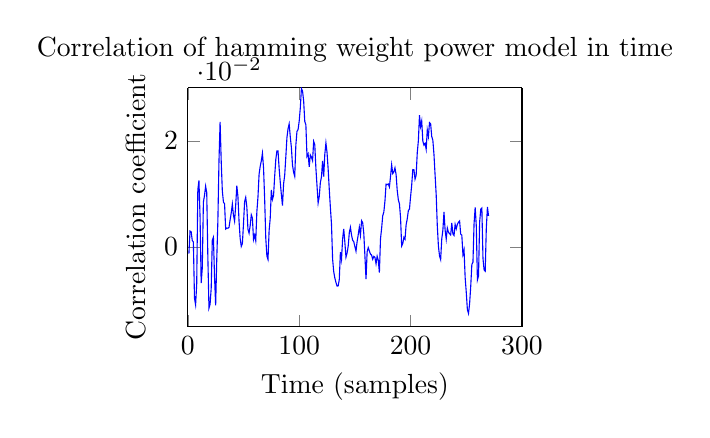
\begin{tikzpicture}

\begin{axis}[%
width=0.35\textwidth,
height=0.25\textwidth,,
at={(0.808889in,0.513333in)},
scale only axis,
separate axis lines,
every outer x axis line/.append style={black},
every x tick label/.append style={font=\color{black}},
xmin=0,
xmax=300,
xlabel={Time (samples)},
every outer y axis line/.append style={black},
every y tick label/.append style={font=\color{black}},
ymin=-0.015,
ymax=0.03,
ylabel={Correlation coefficient},
title={Correlation of hamming weight power model in time}
]
\addplot [color=blue,solid,forget plot]
  table[row sep=crcr]{%
1	-0.00124191773261663\\
2	0.0030113596814982\\
3	0.00289109089867848\\
4	0.00123781070369827\\
5	0.000946988099887706\\
6	-0.00963444456891048\\
7	-0.0109056011278759\\
8	-0.00693908568775801\\
9	0.0107840735377005\\
10	0.0125343776608963\\
11	0.00566982040264624\\
12	-0.00680774801629883\\
13	-0.0039857261866801\\
14	0.00845116032263932\\
15	0.00973204798306401\\
16	0.0114699437140086\\
17	0.0102242980271022\\
18	-0.00188520243615174\\
19	-0.011520990383235\\
20	-0.0107994196744361\\
21	-0.00779826654767437\\
22	0.00127836360759566\\
23	0.00184099855521863\\
24	-0.00561061399013105\\
25	-0.0110238613417115\\
26	-0.00233640502978669\\
27	0.00491525759274175\\
28	0.0162957240373947\\
29	0.0235784489774345\\
30	0.0161311968058564\\
31	0.010577854938711\\
32	0.00847933255520345\\
33	0.00814075206845977\\
34	0.00338920605486348\\
35	0.00357758181192201\\
36	0.00353462925392203\\
37	0.00371033914123386\\
38	0.00513368956680668\\
39	0.00644602160490702\\
40	0.00810143338560267\\
41	0.00594765144431687\\
42	0.00488144389474298\\
43	0.00788758203240359\\
44	0.0115626544397195\\
45	0.0095393978895833\\
46	0.00489084523519676\\
47	0.0016434349561334\\
48	0.000110585378525003\\
49	0.00064212369376973\\
50	0.0043502502868252\\
51	0.00854519292415432\\
52	0.0093547656277726\\
53	0.0075759580881727\\
54	0.00334525961247561\\
55	0.00260739368365825\\
56	0.00401939318844564\\
57	0.00606398367998837\\
58	0.00545671747650534\\
59	0.00139574356078864\\
60	0.00223948171628768\\
61	0.00117639393290399\\
62	0.00664535368435871\\
63	0.00942843442897756\\
64	0.0137394836445989\\
65	0.0152050374130569\\
66	0.0162404709354973\\
67	0.0176702389979158\\
68	0.0149286199194695\\
69	0.00902697241161608\\
70	0.00169534674270825\\
71	-0.00170090513636259\\
72	-0.00236137751348041\\
73	0.00312303886427912\\
74	0.00544256576778266\\
75	0.0107635657109928\\
76	0.00897151525788931\\
77	0.00972964986274892\\
78	0.0133615773465619\\
79	0.0164878422702489\\
80	0.0181110139216583\\
81	0.0180974103658555\\
82	0.0147971413265753\\
83	0.0122360224522456\\
84	0.00988971086424685\\
85	0.00781228758588674\\
86	0.011893444938721\\
87	0.0135579821251652\\
88	0.0169804270891448\\
89	0.0206276522372343\\
90	0.0222882340151556\\
91	0.0232047034746379\\
92	0.0207869299392288\\
93	0.0187463938747807\\
94	0.0154273616867361\\
95	0.014090969845343\\
96	0.0133122515873653\\
97	0.0192029253694727\\
98	0.0217988978932191\\
99	0.0221291846571882\\
100	0.023714742369614\\
101	0.0262075110688421\\
102	0.0298812102452692\\
103	0.029395827675228\\
104	0.0275719947743781\\
105	0.0236841126592988\\
106	0.0230745707301824\\
107	0.0170984254920128\\
108	0.0175613329615171\\
109	0.0151337558018334\\
110	0.017359965898522\\
111	0.0169514169594454\\
112	0.0162865797466159\\
113	0.0198947287357161\\
114	0.0192696502810309\\
115	0.0148477975494898\\
116	0.0115568937642499\\
117	0.00827487217719095\\
118	0.00950553735194381\\
119	0.0121305282915203\\
120	0.0132110607821113\\
121	0.016221619209943\\
122	0.0132699938496486\\
123	0.017461760423934\\
124	0.0196224964573608\\
125	0.0178089702584998\\
126	0.0147178632043674\\
127	0.010908698274486\\
128	0.00745621092976937\\
129	0.00430520214184352\\
130	-0.00229445074267941\\
131	-0.00463806388393287\\
132	-0.00584383423298488\\
133	-0.00668717003628973\\
134	-0.00736562241783064\\
135	-0.00733730561174687\\
136	-0.00613328405343555\\
137	-0.000963440528132496\\
138	-0.00234440088529196\\
139	0.00153726714415262\\
140	0.00342972877119273\\
141	0.000879306751637951\\
142	-0.00191751454386069\\
143	-0.00113280759343479\\
144	0.000165646801663336\\
145	0.00271804058095337\\
146	0.0037041346598561\\
147	0.00224039042791531\\
148	0.00128808306694788\\
149	0.000988697719348249\\
150	8.9761801292765e-05\\
151	-0.000790255444482092\\
152	0.00101504118304252\\
153	0.00230358947036091\\
154	0.00375161175819585\\
155	0.00220319781361994\\
156	0.00496017213796447\\
157	0.00458326128199121\\
158	0.00258186697643241\\
159	-0.00163707894276586\\
160	-0.00606466071647902\\
161	-0.000886345671117554\\
162	-0.000120729691147705\\
163	-0.000765902220651173\\
164	-0.00132455552099588\\
165	-0.00151523532022148\\
166	-0.00230873108163041\\
167	-0.00176492347117222\\
168	-0.00195785092368255\\
169	-0.00316502628396143\\
170	-0.00174031470151016\\
171	-0.00250051816691157\\
172	-0.0048442383672242\\
173	0.00154479777923792\\
174	0.003489420887422\\
175	0.00588981694363952\\
176	0.0066047013568394\\
177	0.00867552177724619\\
178	0.0118487571767962\\
179	0.0117726684930586\\
180	0.0118871092965044\\
181	0.0113115248822237\\
182	0.0133061472422339\\
183	0.0155010005142736\\
184	0.0138377631682439\\
185	0.0141670633649859\\
186	0.0149333226885092\\
187	0.0136628551967338\\
188	0.0106901539638818\\
189	0.00891613188907318\\
190	0.0081262156260998\\
191	0.00554882708633702\\
192	0.000188773855982359\\
193	0.000638565042642912\\
194	0.00182912519553584\\
195	0.00146194110102414\\
196	0.00419242580913252\\
197	0.00528210952063613\\
198	0.00684721699620003\\
199	0.00715148459886334\\
200	0.00948083812227323\\
201	0.0116349390106813\\
202	0.0146002272634951\\
203	0.0145933113233584\\
204	0.0127874378152599\\
205	0.0135011483203399\\
206	0.0177760801932774\\
207	0.0200503882003281\\
208	0.0248390921158618\\
209	0.0226952696941551\\
210	0.0237680512273026\\
211	0.0199705835695962\\
212	0.0192142772463609\\
213	0.0195393179201207\\
214	0.0184200390804313\\
215	0.0220775114553524\\
216	0.0208438183729957\\
217	0.0234521226926168\\
218	0.0232450444027285\\
219	0.0208182208289462\\
220	0.0201331379725087\\
221	0.0174619680724985\\
222	0.0135882200243351\\
223	0.00982326491362919\\
224	0.00397401813164816\\
225	0.000141901213755831\\
226	-0.00169854609445165\\
227	-0.00237724208460807\\
228	0.00153514882408431\\
229	0.00318118431628132\\
230	0.00659913094959573\\
231	0.00322255793069725\\
232	0.00150184307461262\\
233	0.00356748309912564\\
234	0.00275809290490935\\
235	0.00252787453237611\\
236	0.00227568087135651\\
237	0.00452637970640076\\
238	0.00245232879247686\\
239	0.00216681173792444\\
240	0.00425511921157511\\
241	0.00342699651771782\\
242	0.00428385417832136\\
243	0.00466312117151907\\
244	0.0049090152475067\\
245	0.00243430313544051\\
246	0.00224586974842287\\
247	-0.00140734363745939\\
248	-0.00051863732787613\\
249	-0.00578598921261964\\
250	-0.00854277852908817\\
251	-0.0118068677279879\\
252	-0.0125245381309007\\
253	-0.0106753797199441\\
254	-0.00742991762197474\\
255	-0.0033085366870462\\
256	-0.00288477299314674\\
257	0.00443825555692561\\
258	0.00747715112699129\\
259	0.00397046933113535\\
260	-0.00621269406074981\\
261	-0.00545625203895992\\
262	0.0046750592815325\\
263	0.00713684442987915\\
264	0.00734749748562999\\
265	-0.00215008113120001\\
266	-0.00430928584387462\\
267	-0.00456424450346352\\
268	0.00360033000956093\\
269	0.00754387965510516\\
270	0.00587055437017652\\
};
\end{axis}
\end{tikzpicture}%
	\caption{Measured Hamming Distance.}
	\label{fig:cor}
	\end{figure}
  
\section{Conclusion}\label{sec::conclusion} 


% Summarize results and lessons learned.
	Both DPA and CPA have previously been shown to work at recovering secret keys from DES.  We were not able to reproduce such promising results.  We still believe that DPA and CPA should work to recover secret keys from DES but there were some potential flaws in our methods.
	
  	One aspect to this project which could have been done better would have been to take more traces for a single plain text value.  We took 20 traces for each plain text, but we believe that if we had taken many more than this the noise would have averaged out more nicely and the results may have been better.  Perhaps we should have taken an order of magnitude more traces than what we did.  We believe that this was the main contributing factor to the side channel attacks not producing the expected results.
  	
  	We know there is a problem with our data because no correlation is seen to the actual key.  We think the most likely reason is the noise present in the system.  Given more time we might be able to come up with a new experimental setup and method of capturing data that would yield better results.  The lesson learned is that your analysis can only be as good as your data is.  If the data is not good you can't analyze it.
\bibliography{report}
% that's all folks

\section{Apendix A}
DPA and CPA figures :  
  \begin{figure}[]
  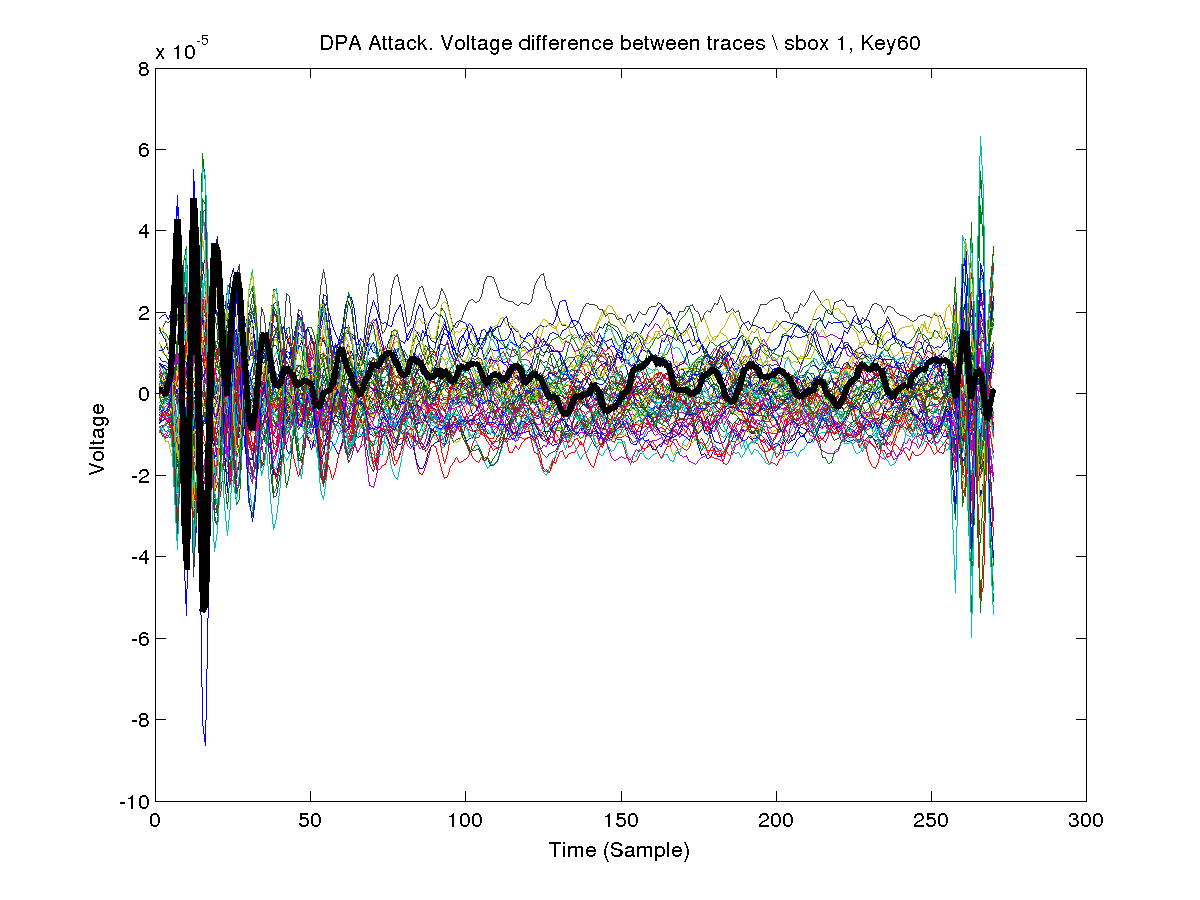
\includegraphics[width=0.9\linewidth]{./dpa1}
  \caption{SBox 1 using DPA.} 
  \label{fig:dpa1}
  \end{figure}
  
  \begin{figure}[]
  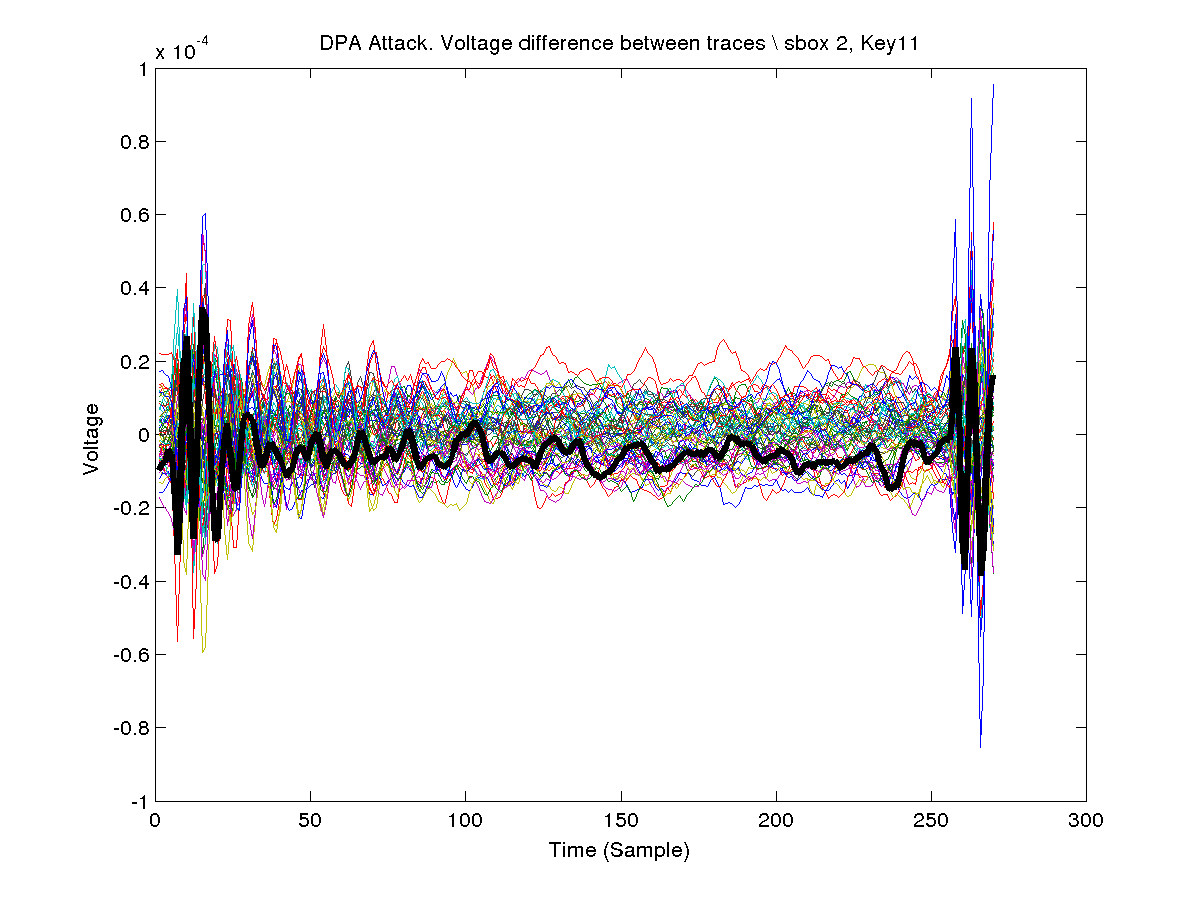
\includegraphics[width=0.9\linewidth]{./dpa2}
  \caption{SBox 2 using DPA.}
  \label{fig:dpa2}
  \end{figure}
  
  \begin{figure}[]
  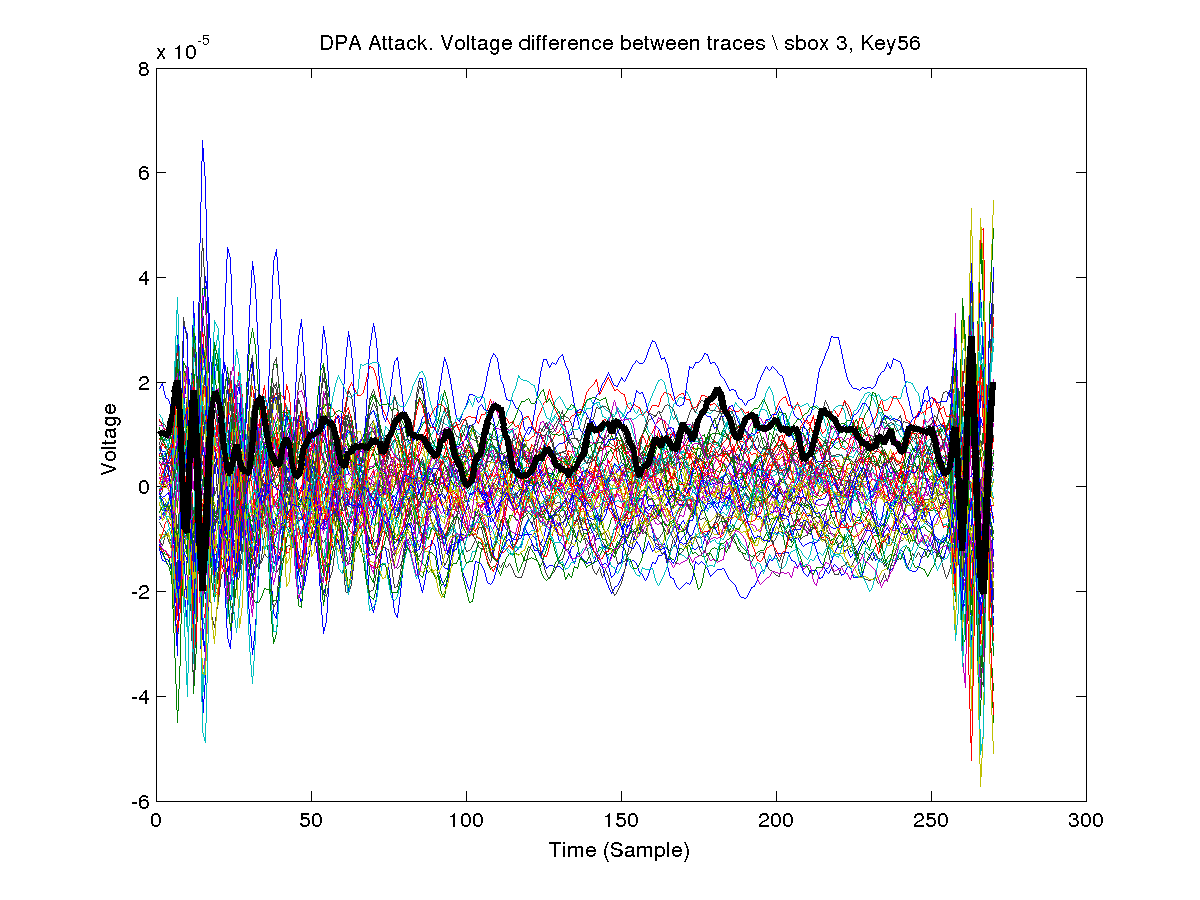
\includegraphics[width=0.9\linewidth]{./dpa3}
  \caption{SBox 3 using DPA.}
  \label{fig:dpa3}
  \end{figure}
  
  \begin{figure}[]
  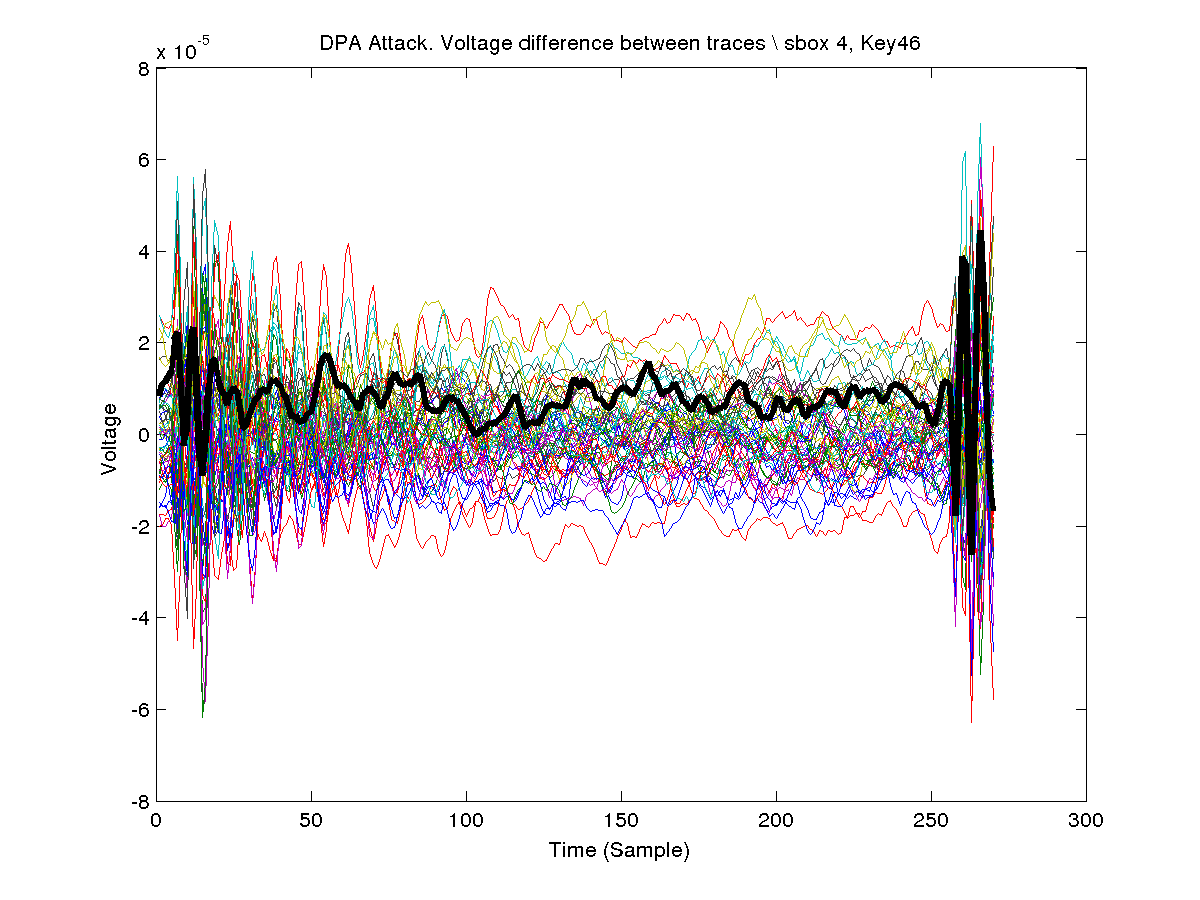
\includegraphics[width=0.9\linewidth]{./dpa4}
  \caption{SBox 4 using DPA.}
  \label{fig:dpa4}
  \end{figure}
  
  \begin{figure}[]
  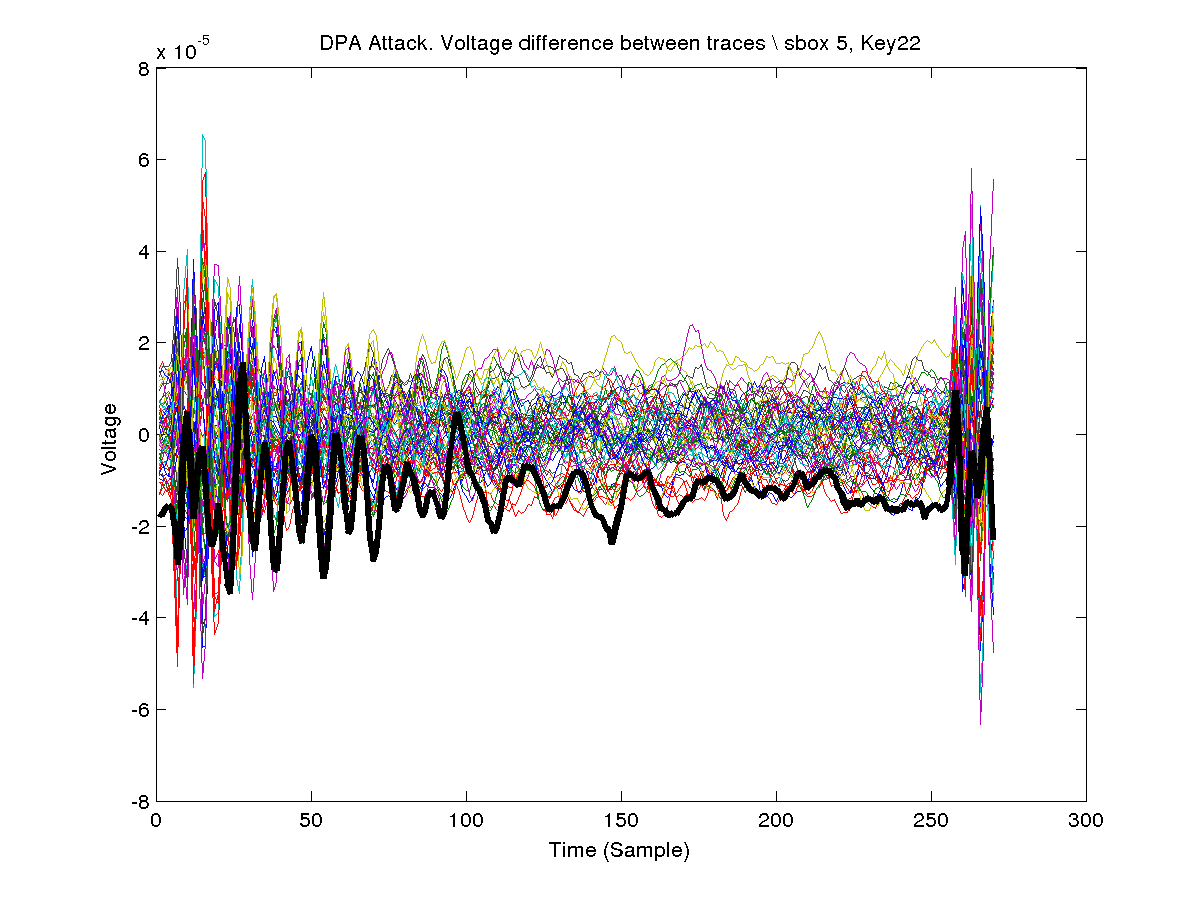
\includegraphics[width=0.9\linewidth]{./dpa5}
  \caption{SBox 5 using DPA.}
  \label{fig:dpa5}
  \end{figure}
  
  \begin{figure}[]
  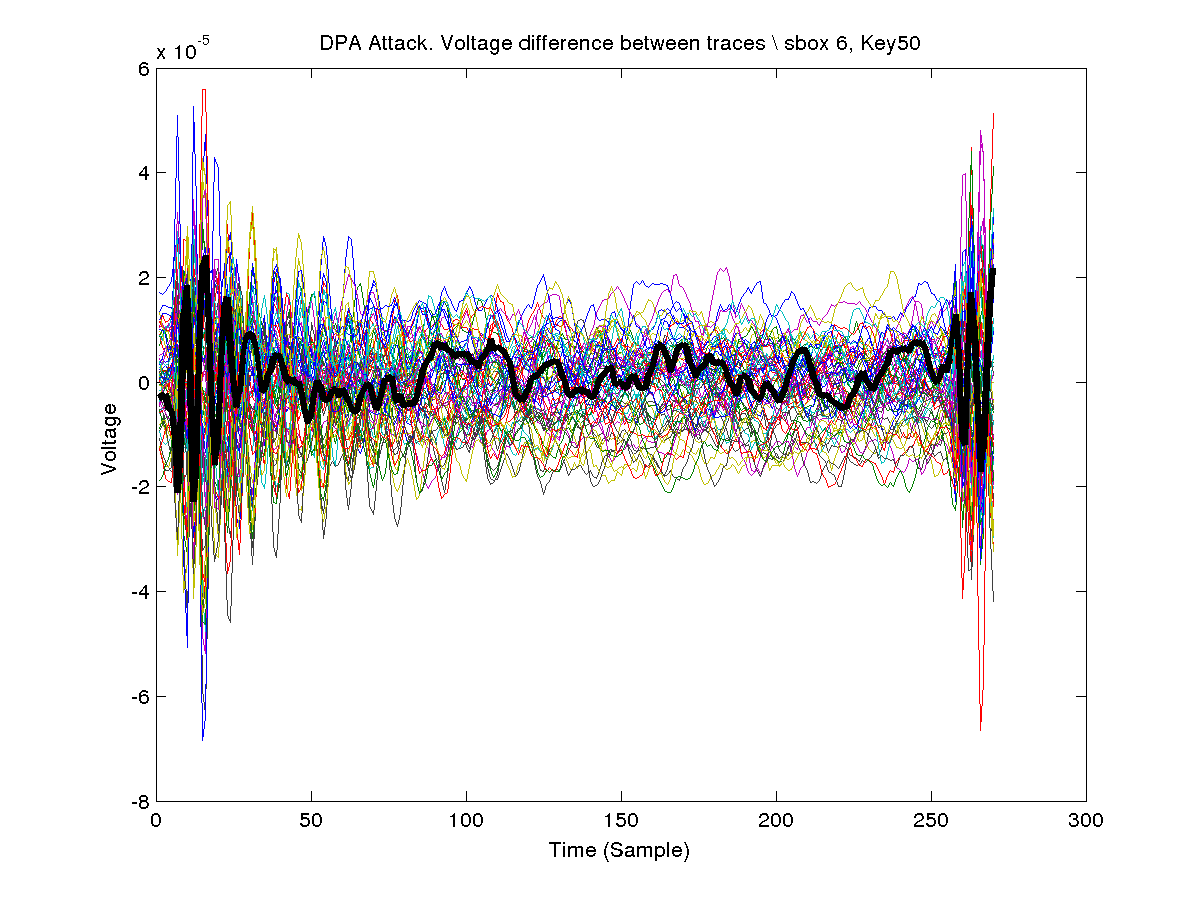
\includegraphics[width=0.9\linewidth]{./dpa6}
  \caption{SBox 6 using DPA.}
  \label{fig:dpa6}
  \end{figure}
  
  \begin{figure}[]
  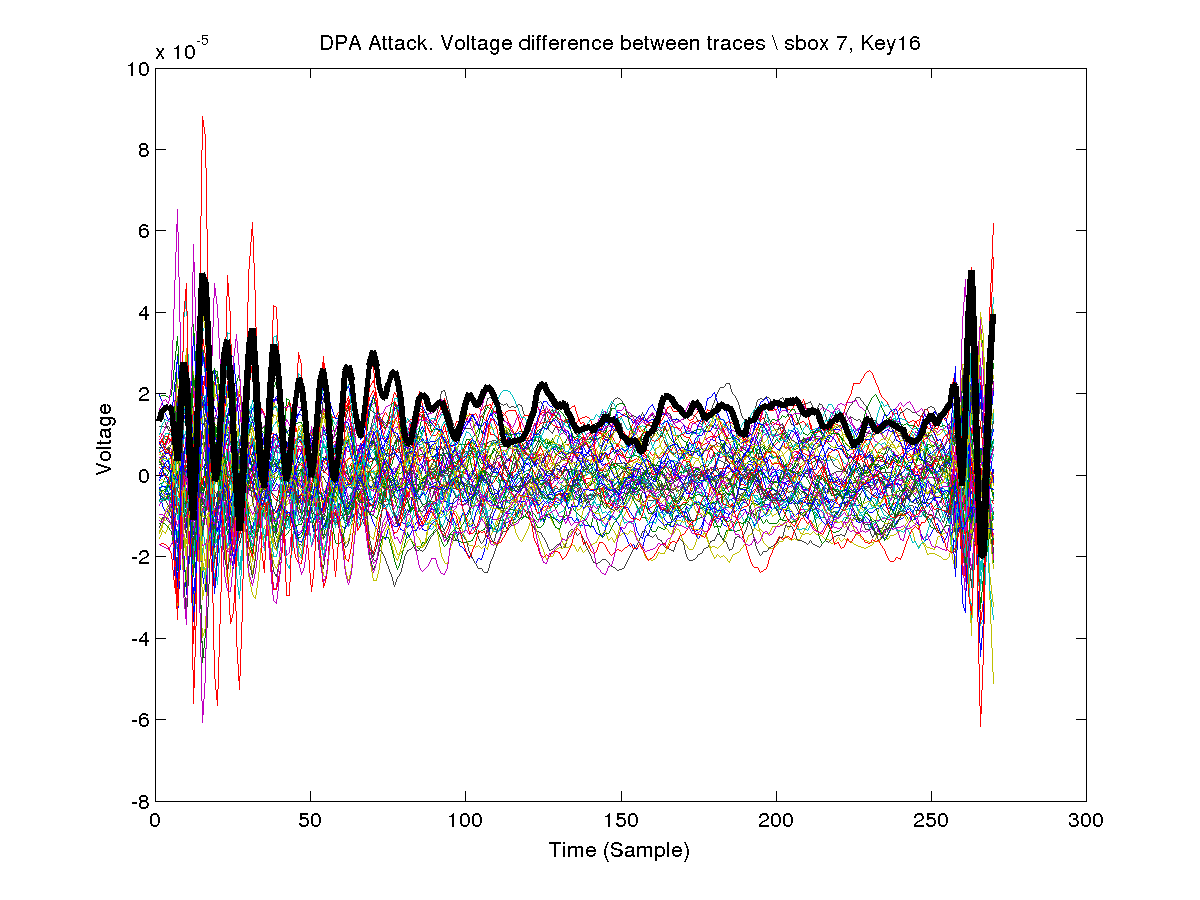
\includegraphics[width=0.9\linewidth]{./dpa7}
  \caption{SBox 7 using DPA.}
  \label{fig:dpa7}
  \end{figure}
  
  \begin{figure}[]
  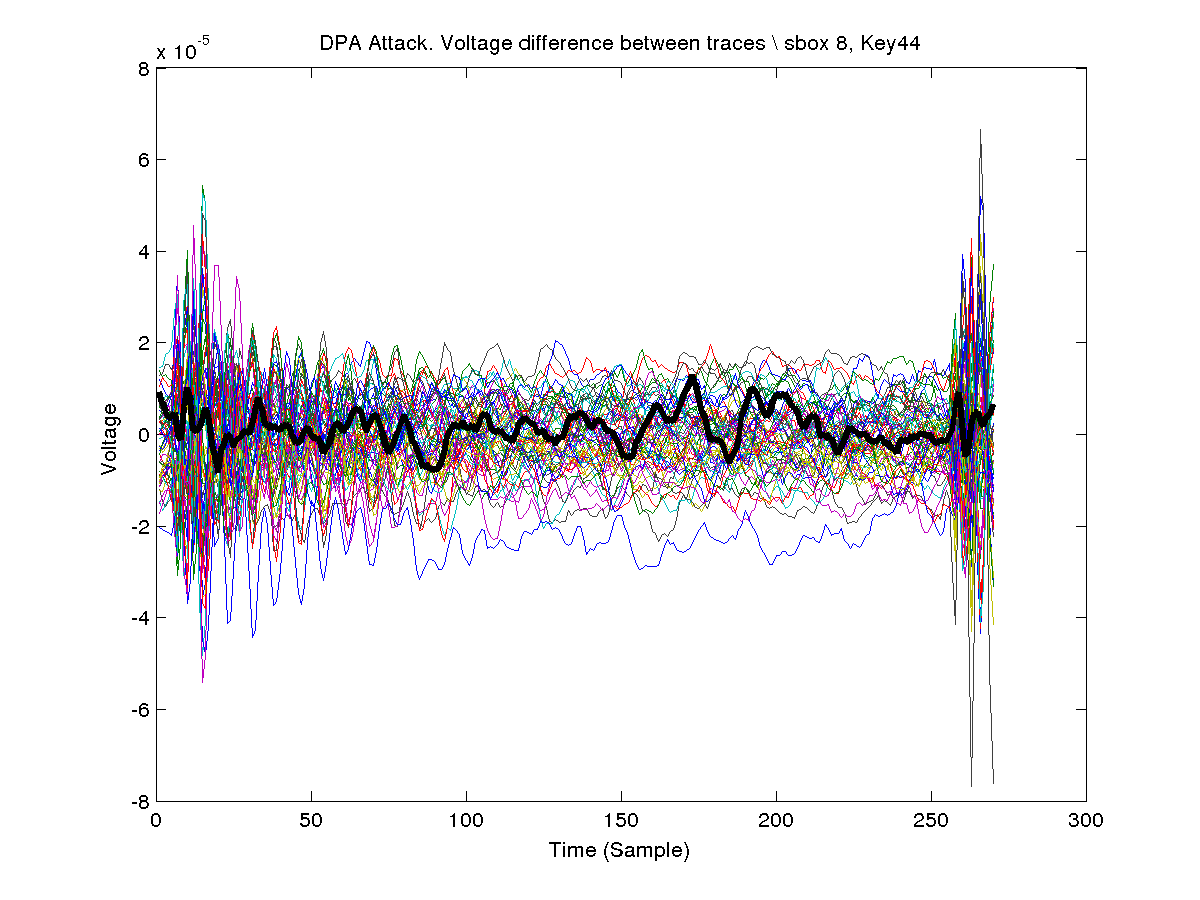
\includegraphics[width=0.9\linewidth]{./dpa8}
  \caption{SBox 8 using DPA.}
  \label{fig:dpa8}
  \end{figure}
  
  \begin{figure}[]
  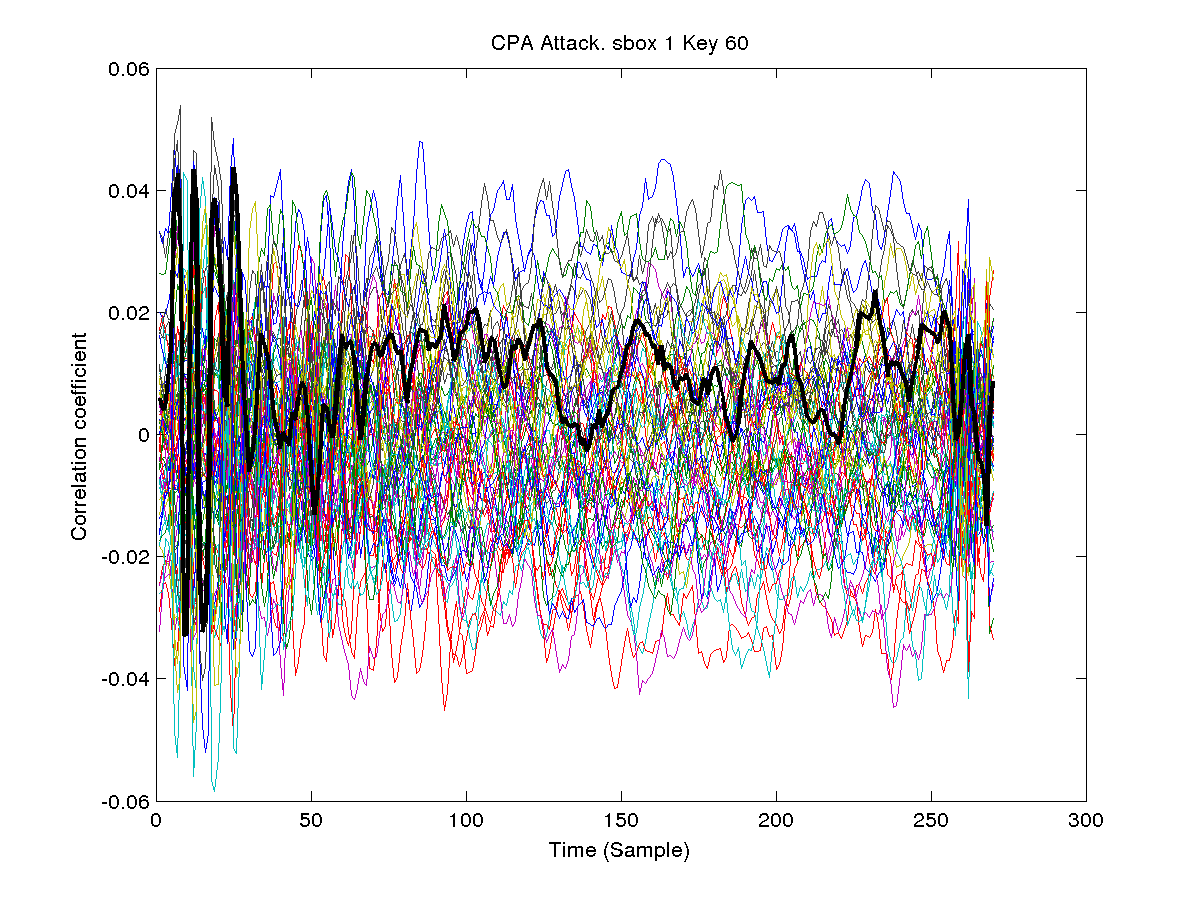
\includegraphics[width=0.9\linewidth]{./cpa1}
  \caption{SBox 1 using CPA.}
  \label{fig:cpa1}
  \end{figure}

  \begin{figure}[]
  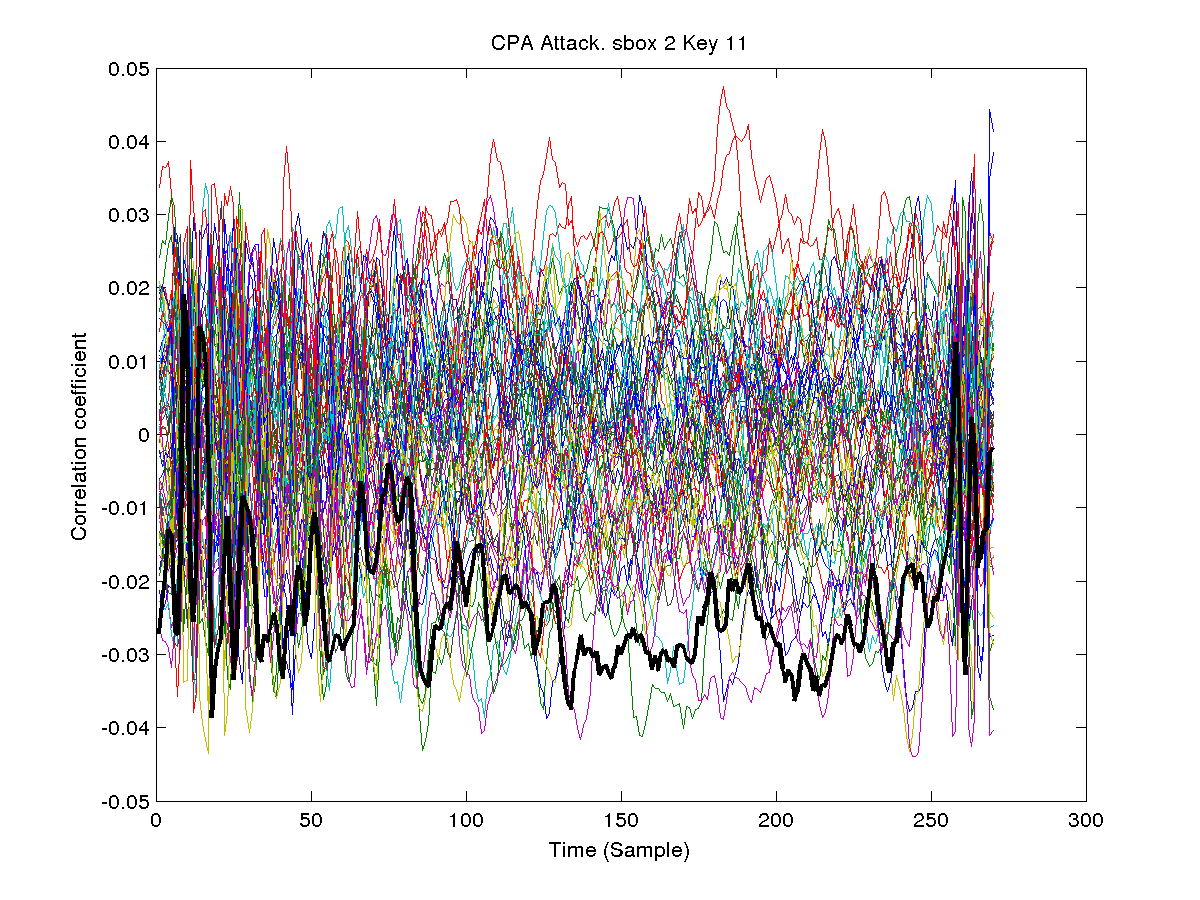
\includegraphics[width=0.9\linewidth]{./cpa2}
  \caption{SBox 2 using CPA.}
  \label{fig:cpa2}
  \end{figure}

  \begin{figure}[]
  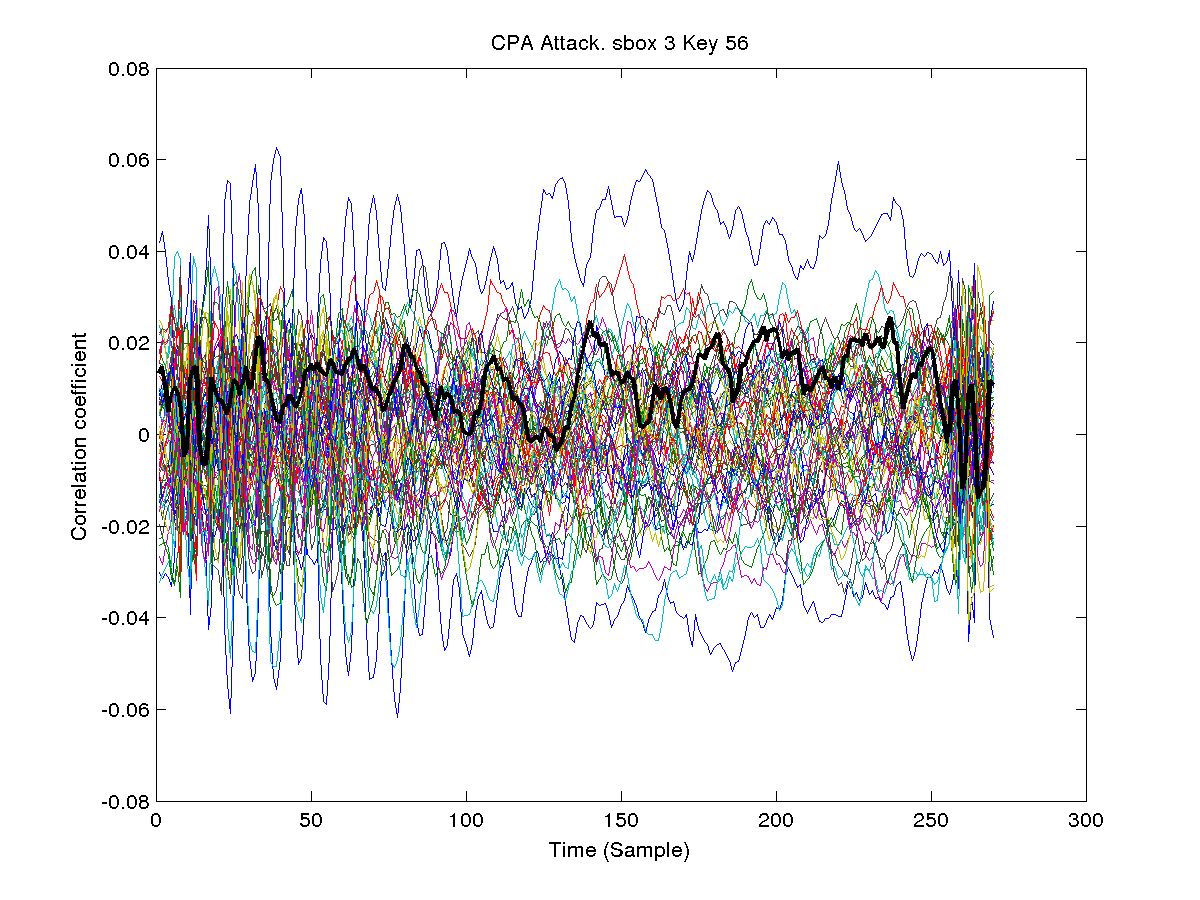
\includegraphics[width=0.9\linewidth]{./cpa3}
  \caption{SBox 3 using CPA.}
  \label{fig:cpa3}
  \end{figure}

  \begin{figure}[]
  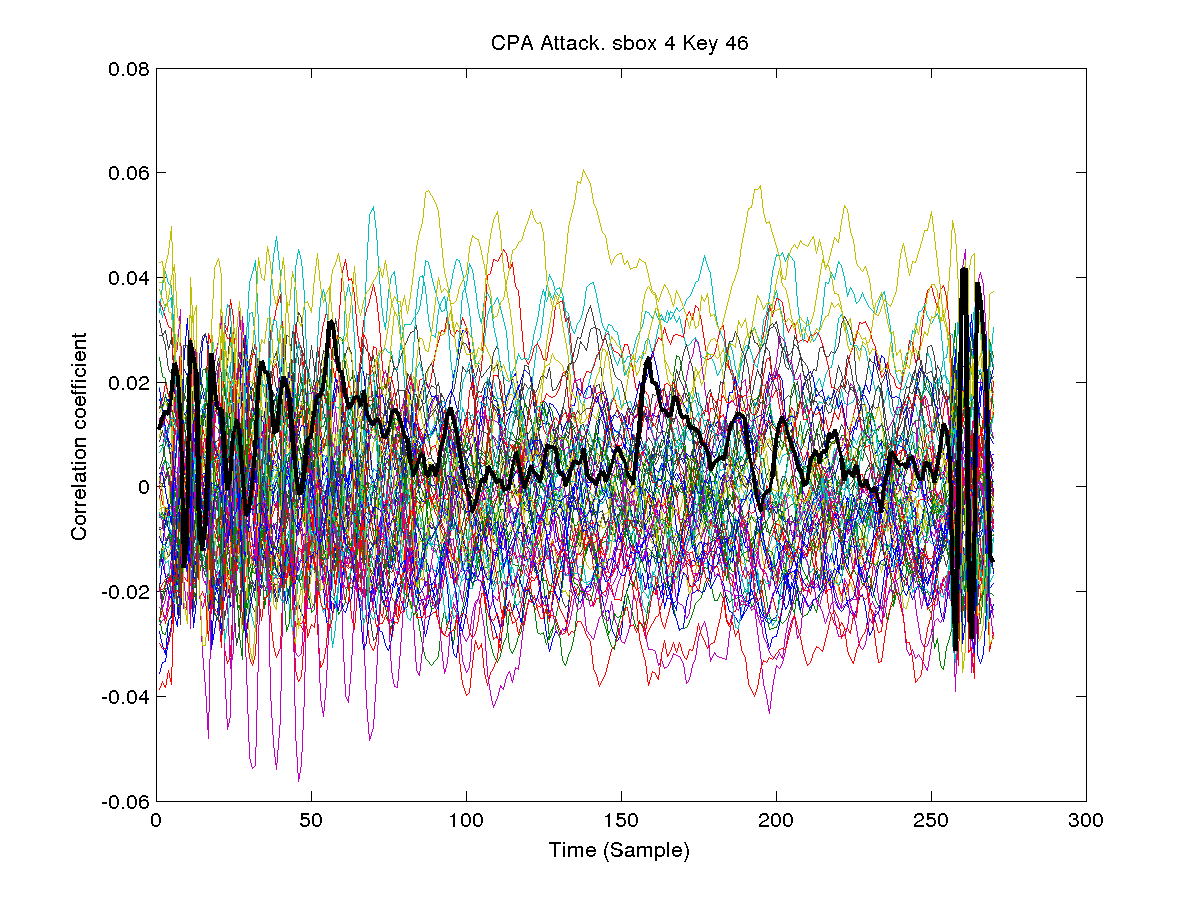
\includegraphics[width=0.9\linewidth]{./cpa4}
  \caption{SBox 4 using CPA.}
  \label{fig:cpa4}
  \end{figure}

  \begin{figure}[]
  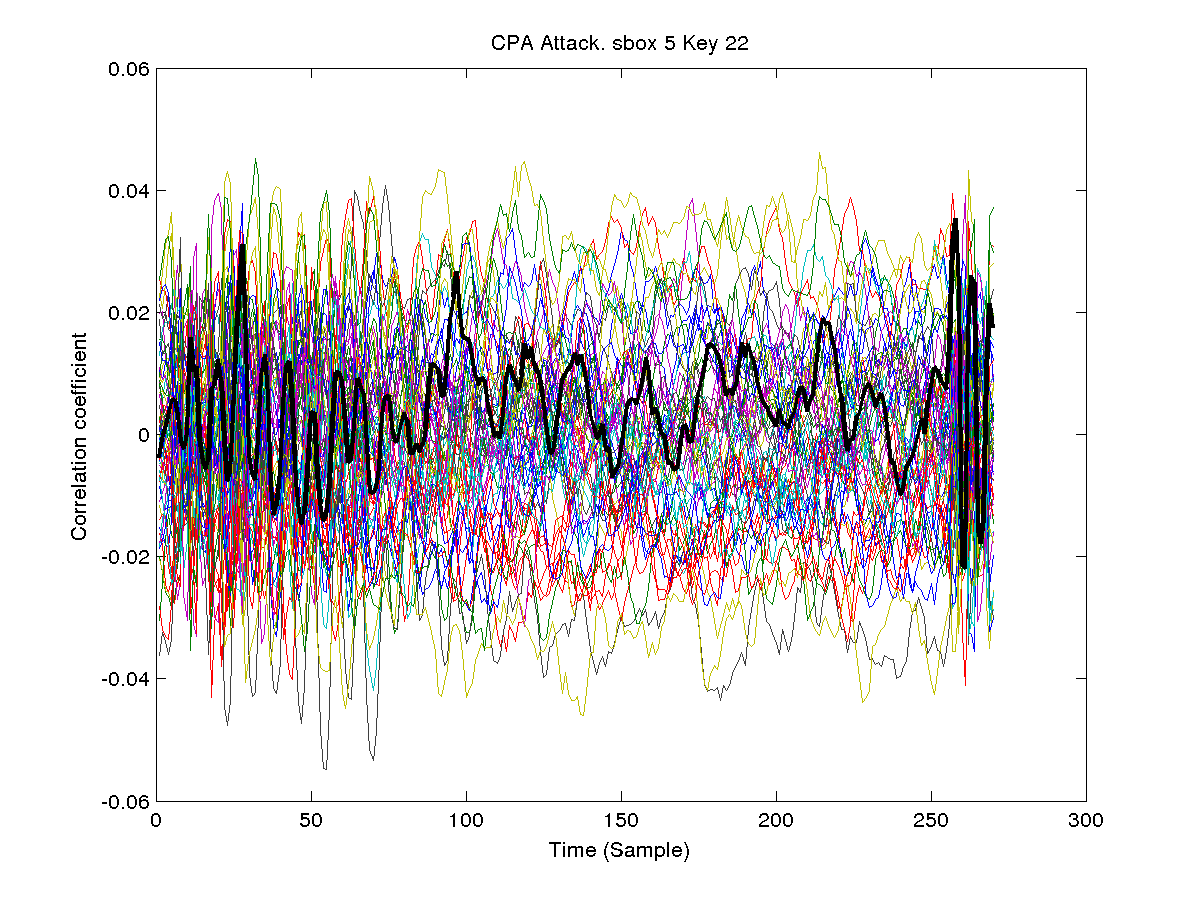
\includegraphics[width=0.9\linewidth]{./cpa5}
  \caption{SBox 5 using CPA.}
  \label{fig:cpa5}
  \end{figure}

  \begin{figure}[]
  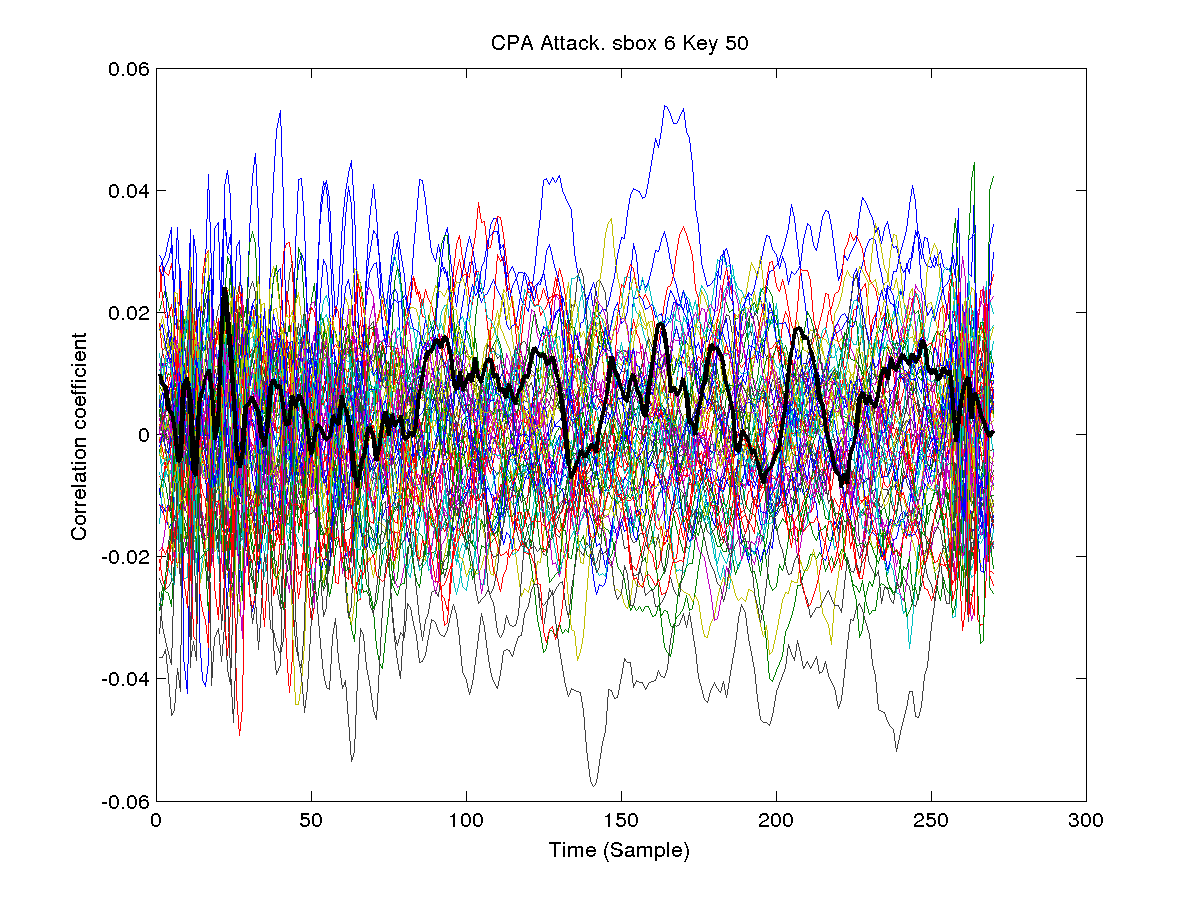
\includegraphics[width=0.9\linewidth]{./cpa6}
  \caption{SBox 6 using CPA.}
  \label{fig:cpa6}
  \end{figure}

  \begin{figure}[]
  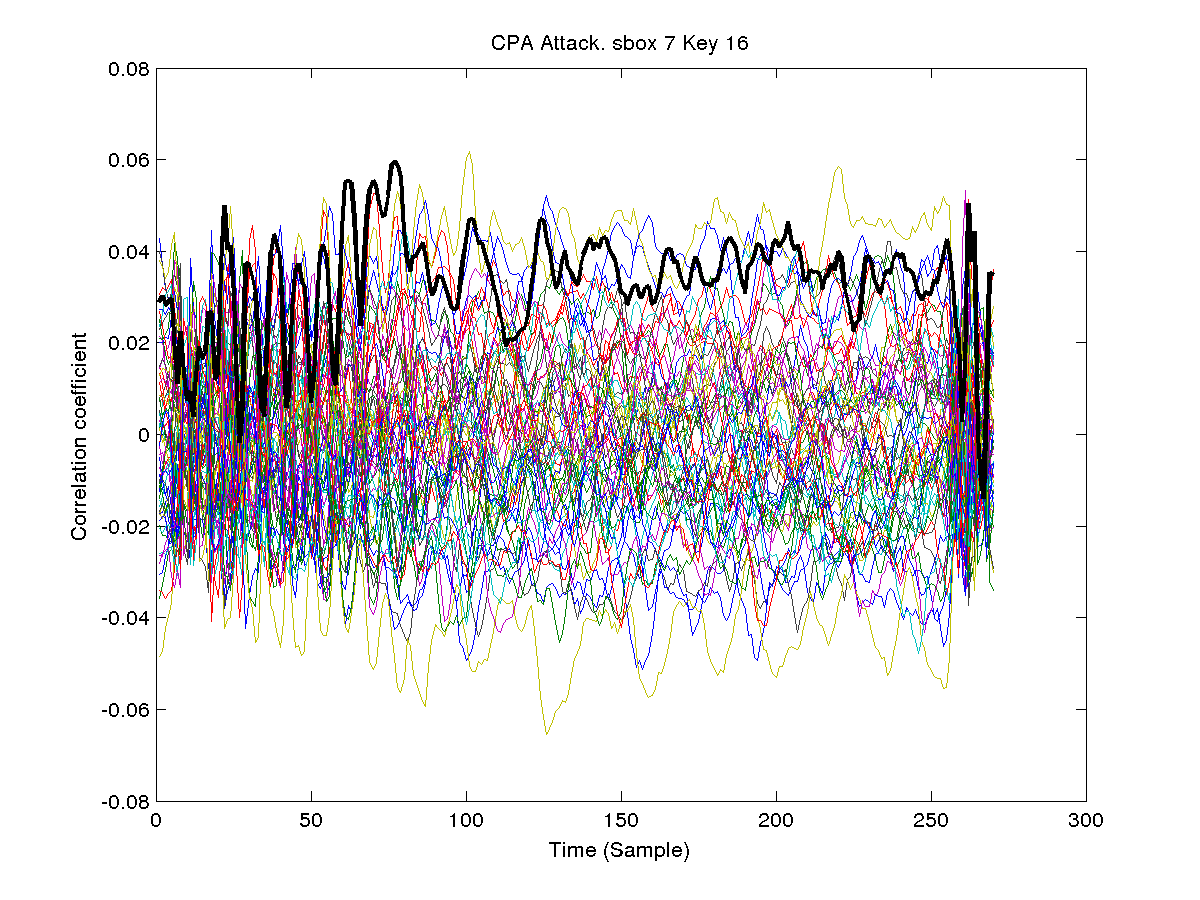
\includegraphics[width=0.9\linewidth]{./cpa7}
  \caption{SBox 7 using CPA.}
  \label{fig:cpa7}
  \end{figure}

  \begin{figure}[]
  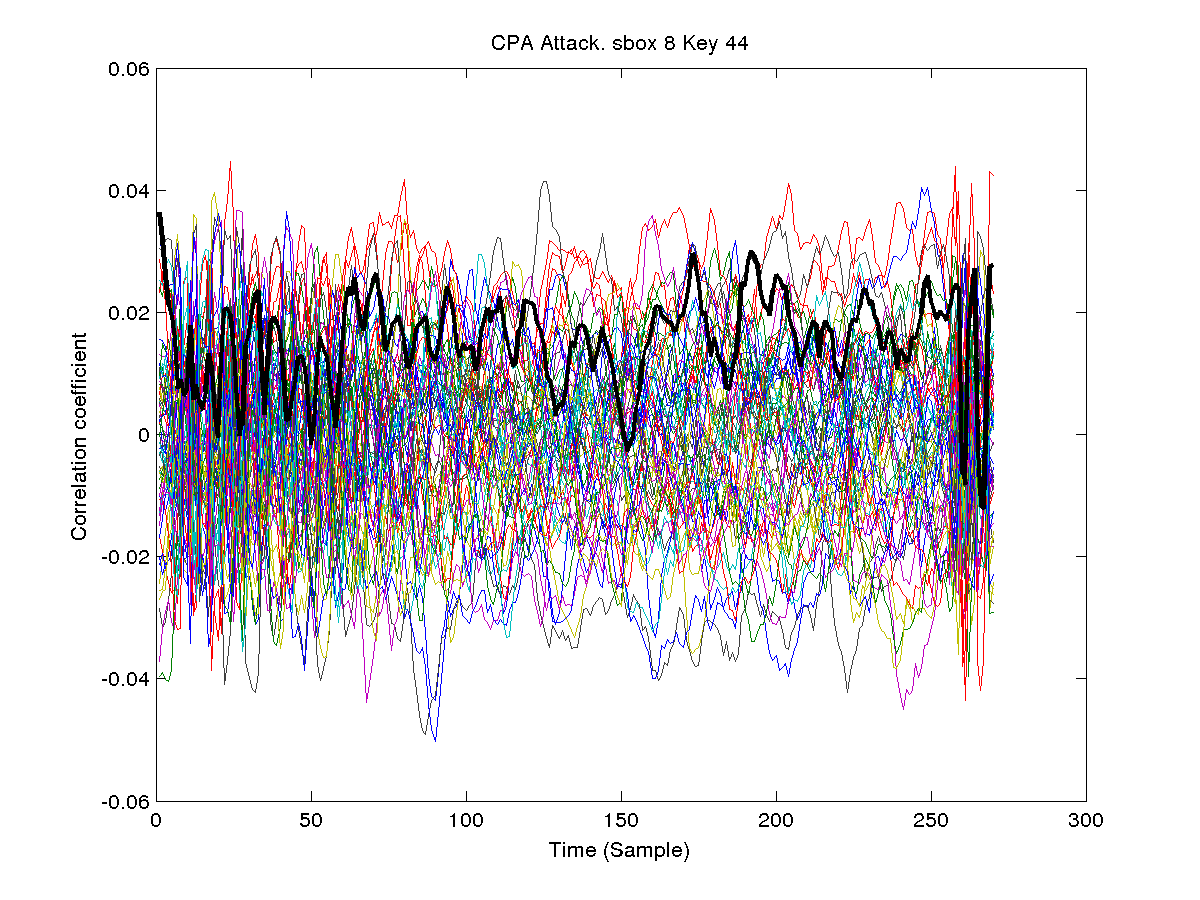
\includegraphics[width=0.9\linewidth]{./cpa8}
  \caption{SBox 8 using CPA.}
  \label{fig:cpa8}
  \end{figure}	

\end{document}






